% Options for packages loaded elsewhere
\PassOptionsToPackage{unicode}{hyperref}
\PassOptionsToPackage{hyphens}{url}
\PassOptionsToPackage{dvipsnames,svgnames*,x11names*}{xcolor}
%
\documentclass[
  8pt,
  ignorenonframetext,
  dvipsnames]{beamer}
\usepackage{pgfpages}
\setbeamertemplate{caption}[numbered]
\setbeamertemplate{caption label separator}{: }
\setbeamercolor{caption name}{fg=normal text.fg}
\beamertemplatenavigationsymbolsempty
% Prevent slide breaks in the middle of a paragraph
\widowpenalties 1 10000
\raggedbottom
\setbeamertemplate{part page}{
  \centering
  \begin{beamercolorbox}[sep=16pt,center]{part title}
    \usebeamerfont{part title}\insertpart\par
  \end{beamercolorbox}
}
\setbeamertemplate{section page}{
  \centering
  \begin{beamercolorbox}[sep=12pt,center]{part title}
    \usebeamerfont{section title}\insertsection\par
  \end{beamercolorbox}
}
\setbeamertemplate{subsection page}{
  \centering
  \begin{beamercolorbox}[sep=8pt,center]{part title}
    \usebeamerfont{subsection title}\insertsubsection\par
  \end{beamercolorbox}
}
\AtBeginPart{
  \frame{\partpage}
}
\AtBeginSection{
  \ifbibliography
  \else
    \frame{\sectionpage}
  \fi
}
\AtBeginSubsection{
  \frame{\subsectionpage}
}
\usepackage{lmodern}
\usepackage{amssymb,amsmath}
\usepackage{ifxetex,ifluatex}
\ifnum 0\ifxetex 1\fi\ifluatex 1\fi=0 % if pdftex
  \usepackage[T1]{fontenc}
  \usepackage[utf8]{inputenc}
  \usepackage{textcomp} % provide euro and other symbols
\else % if luatex or xetex
  \usepackage{unicode-math}
  \defaultfontfeatures{Scale=MatchLowercase}
  \defaultfontfeatures[\rmfamily]{Ligatures=TeX,Scale=1}
\fi
% Use upquote if available, for straight quotes in verbatim environments
\IfFileExists{upquote.sty}{\usepackage{upquote}}{}
\IfFileExists{microtype.sty}{% use microtype if available
  \usepackage[]{microtype}
  \UseMicrotypeSet[protrusion]{basicmath} % disable protrusion for tt fonts
}{}
\makeatletter
\@ifundefined{KOMAClassName}{% if non-KOMA class
  \IfFileExists{parskip.sty}{%
    \usepackage{parskip}
  }{% else
    \setlength{\parindent}{0pt}
    \setlength{\parskip}{6pt plus 2pt minus 1pt}}
}{% if KOMA class
  \KOMAoptions{parskip=half}}
\makeatother
\usepackage{xcolor}
\IfFileExists{xurl.sty}{\usepackage{xurl}}{} % add URL line breaks if available
\IfFileExists{bookmark.sty}{\usepackage{bookmark}}{\usepackage{hyperref}}
\hypersetup{
  pdftitle={Introduction to R and R data structures},
  pdfauthor={Ozan Jaquette},
  colorlinks=true,
  linkcolor=Maroon,
  filecolor=Maroon,
  citecolor=Blue,
  urlcolor=blue,
  pdfcreator={LaTeX via pandoc}}
\urlstyle{same} % disable monospaced font for URLs
\newif\ifbibliography
\usepackage{color}
\usepackage{fancyvrb}
\newcommand{\VerbBar}{|}
\newcommand{\VERB}{\Verb[commandchars=\\\{\}]}
\DefineVerbatimEnvironment{Highlighting}{Verbatim}{commandchars=\\\{\}}
% Add ',fontsize=\small' for more characters per line
\usepackage{framed}
\definecolor{shadecolor}{RGB}{248,248,248}
\newenvironment{Shaded}{\begin{snugshade}}{\end{snugshade}}
\newcommand{\AlertTok}[1]{\textcolor[rgb]{0.94,0.16,0.16}{#1}}
\newcommand{\AnnotationTok}[1]{\textcolor[rgb]{0.56,0.35,0.01}{\textbf{\textit{#1}}}}
\newcommand{\AttributeTok}[1]{\textcolor[rgb]{0.77,0.63,0.00}{#1}}
\newcommand{\BaseNTok}[1]{\textcolor[rgb]{0.00,0.00,0.81}{#1}}
\newcommand{\BuiltInTok}[1]{#1}
\newcommand{\CharTok}[1]{\textcolor[rgb]{0.31,0.60,0.02}{#1}}
\newcommand{\CommentTok}[1]{\textcolor[rgb]{0.56,0.35,0.01}{\textit{#1}}}
\newcommand{\CommentVarTok}[1]{\textcolor[rgb]{0.56,0.35,0.01}{\textbf{\textit{#1}}}}
\newcommand{\ConstantTok}[1]{\textcolor[rgb]{0.00,0.00,0.00}{#1}}
\newcommand{\ControlFlowTok}[1]{\textcolor[rgb]{0.13,0.29,0.53}{\textbf{#1}}}
\newcommand{\DataTypeTok}[1]{\textcolor[rgb]{0.13,0.29,0.53}{#1}}
\newcommand{\DecValTok}[1]{\textcolor[rgb]{0.00,0.00,0.81}{#1}}
\newcommand{\DocumentationTok}[1]{\textcolor[rgb]{0.56,0.35,0.01}{\textbf{\textit{#1}}}}
\newcommand{\ErrorTok}[1]{\textcolor[rgb]{0.64,0.00,0.00}{\textbf{#1}}}
\newcommand{\ExtensionTok}[1]{#1}
\newcommand{\FloatTok}[1]{\textcolor[rgb]{0.00,0.00,0.81}{#1}}
\newcommand{\FunctionTok}[1]{\textcolor[rgb]{0.00,0.00,0.00}{#1}}
\newcommand{\ImportTok}[1]{#1}
\newcommand{\InformationTok}[1]{\textcolor[rgb]{0.56,0.35,0.01}{\textbf{\textit{#1}}}}
\newcommand{\KeywordTok}[1]{\textcolor[rgb]{0.13,0.29,0.53}{\textbf{#1}}}
\newcommand{\NormalTok}[1]{#1}
\newcommand{\OperatorTok}[1]{\textcolor[rgb]{0.81,0.36,0.00}{\textbf{#1}}}
\newcommand{\OtherTok}[1]{\textcolor[rgb]{0.56,0.35,0.01}{#1}}
\newcommand{\PreprocessorTok}[1]{\textcolor[rgb]{0.56,0.35,0.01}{\textit{#1}}}
\newcommand{\RegionMarkerTok}[1]{#1}
\newcommand{\SpecialCharTok}[1]{\textcolor[rgb]{0.00,0.00,0.00}{#1}}
\newcommand{\SpecialStringTok}[1]{\textcolor[rgb]{0.31,0.60,0.02}{#1}}
\newcommand{\StringTok}[1]{\textcolor[rgb]{0.31,0.60,0.02}{#1}}
\newcommand{\VariableTok}[1]{\textcolor[rgb]{0.00,0.00,0.00}{#1}}
\newcommand{\VerbatimStringTok}[1]{\textcolor[rgb]{0.31,0.60,0.02}{#1}}
\newcommand{\WarningTok}[1]{\textcolor[rgb]{0.56,0.35,0.01}{\textbf{\textit{#1}}}}
\usepackage{longtable,booktabs}
\usepackage{caption}
% Make caption package work with longtable
\makeatletter
\def\fnum@table{\tablename~\thetable}
\makeatother
\usepackage{graphicx}
\makeatletter
\def\maxwidth{\ifdim\Gin@nat@width>\linewidth\linewidth\else\Gin@nat@width\fi}
\def\maxheight{\ifdim\Gin@nat@height>\textheight\textheight\else\Gin@nat@height\fi}
\makeatother
% Scale images if necessary, so that they will not overflow the page
% margins by default, and it is still possible to overwrite the defaults
% using explicit options in \includegraphics[width, height, ...]{}
\setkeys{Gin}{width=\maxwidth,height=\maxheight,keepaspectratio}
% Set default figure placement to htbp
\makeatletter
\def\fps@figure{htbp}
\makeatother
\setlength{\emergencystretch}{3em} % prevent overfull lines
\providecommand{\tightlist}{%
  \setlength{\itemsep}{0pt}\setlength{\parskip}{0pt}}
\setcounter{secnumdepth}{-\maxdimen} % remove section numbering

%packages
\usepackage{graphicx}
\usepackage{rotating}
\usepackage{hyperref}

\usepackage{tikz} % used for text highlighting, amongst others
\usepackage{comment}

%title slide stuff
%\institute{Department of Education}
%\title{Managing and Manipulating Data Using R}

%
\setbeamertemplate{navigation symbols}{} % get rid of navigation icons:
\setbeamertemplate{footline}[page number]

%\setbeamertemplate{frametitle}{\thesection \hspace{0.2cm} \insertframetitle}
\setbeamertemplate{section in toc}[sections numbered]
%\setbeamertemplate{subsection in toc}[subsections numbered]
\setbeamertemplate{subsection in toc}{%
  \leavevmode\leftskip=3.2em\color{gray}\rlap{\hskip-2em\inserttocsectionnumber.\inserttocsubsectionnumber}\inserttocsubsection\par
}

%define colors
%\definecolor{uva_orange}{RGB}{216,141,42} % UVa orange (Rotunda orange)
\definecolor{mygray}{rgb}{0.95, 0.95, 0.95} % for highlighted text
	% grey is equal parts red, green, blue. higher values >> lighter grey
	%\definecolor{lightgraybo}{rgb}{0.83, 0.83, 0.83}

% new commands

%highlight text with very light grey
\newcommand*{\hlg}[1]{%
	\tikz[baseline=(X.base)] \node[rectangle, fill=mygray] (X) {#1};%
}
%, inner sep=0.3mm
%highlight text with very light grey and use font associated with code
\newcommand*{\hlgc}[1]{\texttt{\hlg{#1}}}

%modifying back ticks to add grey background
\let\OldTexttt\texttt
\renewcommand{\texttt}[1]{\OldTexttt{\hlg{#1}}}


\begin{comment}

% Font
\usepackage[defaultfam,light,tabular,lining]{montserrat}
\usepackage[T1]{fontenc}
\renewcommand*\oldstylenums[1]{{\fontfamily{Montserrat-TOsF}\selectfont #1}}

% Change color of boldface text to darkgray
\renewcommand{\textbf}[1]{{\color{darkgray}\bfseries\fontfamily{Montserrat-TOsF}#1}}

% Bullet points
\setbeamertemplate{itemize item}{\color{BlueViolet}$\circ$}
\setbeamertemplate{itemize subitem}{\color{BrickRed}$\triangleright$}
\setbeamertemplate{itemize subsubitem}{$-$}

% Reduce space before lists
%\addtobeamertemplate{itemize/enumerate body begin}{}{\vspace*{-8pt}}

\let\olditem\item
\renewcommand{\item}{%
  \olditem\vspace{4pt}
}

% decreasing space before and after level-2 bullet block
%\addtobeamertemplate{itemize/enumerate subbody begin}{}{\vspace*{-3pt}}
%\addtobeamertemplate{itemize/enumerate subbody end}{}{\vspace*{-3pt}}

% decreasing space before and after level-3 bullet block
%\addtobeamertemplate{itemize/enumerate subsubbody begin}{}{\vspace*{-2pt}}
%\addtobeamertemplate{itemize/enumerate subsubbody end}{}{\vspace*{-2pt}}

%Section numbering
\setbeamertemplate{section page}{%
    \begingroup
        \begin{beamercolorbox}[sep=10pt,center,rounded=true,shadow=true]{section title}
        \usebeamerfont{section title}\thesection~\insertsection\par
        \end{beamercolorbox}
    \endgroup
}

\setbeamertemplate{subsection page}{%
    \begingroup
        \begin{beamercolorbox}[sep=6pt,center,rounded=true,shadow=true]{subsection title}
        \usebeamerfont{subsection title}\thesection.\thesubsection~\insertsubsection\par
        \end{beamercolorbox}
    \endgroup
}

\end{comment}
\ifluatex
  \usepackage{selnolig}  % disable illegal ligatures
\fi

\title{Introduction to R and R data structures}
\subtitle{EDUC 263: Introduction to Programming and Data Management
Using R}
\author{Ozan Jaquette}
\date{}

\begin{document}
\frame{\titlepage}

\begin{frame}[allowframebreaks]
  \tableofcontents[hideallsubsections]
\end{frame}
\hypertarget{what-is-r-why-r}{%
\section{What is R? Why R?}\label{what-is-r-why-r}}

\begin{frame}{What is R?}
\protect\hypertarget{what-is-r}{}
According to the Inter-University Consortium for Political and Social
Research
\href{https://www.icpsr.umich.edu/icpsrweb/content/shared/ICPSR/faqs/what-is-r.html}{(ICPSR)}:

\medskip

\begin{quote}
R is ``an alternative to traditional statistical packages such as SPSS,
SAS, and Stata such that it is an extensible, open-source language and
computing environment for Windows, Macintosh, UNIX, and Linux platforms.
Such software allows for the user to freely distribute, study, change,
and improve the software under the
\href{https://www.gnu.org/home.en.html}{Free Software Foundation's GNU
General Public License}.''
\end{quote}

\medskip

For more info visit
\href{https://www.r-project.org/about.html}{R-project.org}
\end{frame}

\begin{frame}[fragile]{Base R vs.~R packages}
\protect\hypertarget{base-r-vs.-r-packages}{}
Base R

\begin{itemize}
\tightlist
\item
  When you install R, you automatically install the
  \href{https://stat.ethz.ch/R-manual/R-devel/library/base/html/00Index.html}{``Base
  R''} set of functions
\item
  Example of a few of the functions in in Base R:

  \begin{itemize}
  \tightlist
  \item
    \texttt{as.character()} function
  \item
    \texttt{print()} function
  \item
    \texttt{setwd()} function
  \end{itemize}
\end{itemize}

\medskip

R packages

\begin{itemize}
\tightlist
\item
  an R ``package'' (or ``library'') is a collection of (related)
  functions developed by the R community
\item
  Examples of R packages:

  \begin{itemize}
  \tightlist
  \item
    \texttt{tidyverse} package for manipulating and visualizing data
  \item
    \texttt{igraph} package for network analyses
  \item
    \texttt{leaflet} package for mapping
  \item
    \texttt{rvest} package for webscraping
  \item
    \texttt{rtweet} package for streaming and downloading data from
    Twitter
  \end{itemize}
\item
  \textbf{All} R packages are free! More about R packages in later
  weeks\ldots{}
\end{itemize}
\end{frame}

\begin{frame}[fragile]{Installing and Loading R packages}
\protect\hypertarget{installing-and-loading-r-packages}{}
You only need to install a package once. To install an R package use
\texttt{install.package()} function.

\begin{Shaded}
\begin{Highlighting}[]
\CommentTok{\#install.packages("tidyverse")}
\end{Highlighting}
\end{Shaded}

You need to load a package everytime you plan to use it. To load a
package use the \texttt{library()} function.

\begin{Shaded}
\begin{Highlighting}[]
\KeywordTok{library}\NormalTok{(tidyverse)}
\CommentTok{\#\textgreater{} {-}{-} Attaching packages {-}{-}{-}{-}{-}{-}{-}{-}{-}{-}{-}{-}{-}{-}{-}{-}{-}{-}{-}{-}{-}{-}{-}{-}{-}{-}{-}{-}{-}{-}{-}{-}{-}{-}{-}{-}{-}{-}{-}{-}{-}{-}{-}{-}{-}{-}{-}{-}{-}{-}{-}{-} tidyverse 1.3.0 {-}{-}}
\CommentTok{\#\textgreater{} v ggplot2 3.3.2     v purrr   0.3.4}
\CommentTok{\#\textgreater{} v tibble  3.0.3     v dplyr   1.0.2}
\CommentTok{\#\textgreater{} v tidyr   1.1.2     v stringr 1.4.0}
\CommentTok{\#\textgreater{} v readr   1.3.1     v forcats 0.5.0}
\CommentTok{\#\textgreater{} {-}{-} Conflicts {-}{-}{-}{-}{-}{-}{-}{-}{-}{-}{-}{-}{-}{-}{-}{-}{-}{-}{-}{-}{-}{-}{-}{-}{-}{-}{-}{-}{-}{-}{-}{-}{-}{-}{-}{-}{-}{-}{-}{-}{-}{-}{-}{-}{-}{-}{-}{-}{-}{-}{-}{-}{-}{-}{-} tidyverse\_conflicts() {-}{-}}
\CommentTok{\#\textgreater{} x dplyr::filter() masks stats::filter()}
\CommentTok{\#\textgreater{} x dplyr::lag()    masks stats::lag()}
\end{Highlighting}
\end{Shaded}
\end{frame}

\begin{frame}{RStudio}
\protect\hypertarget{rstudio}{}
``\href{https://www.rstudio.com/products/rstudio/features/}{RStudio} is
an integrated development environment (IDE) for R. It includes a
console, syntax-highlighting editor that supports direct code execution,
as well as tools for plotting, history, debugging and workspace
management.''

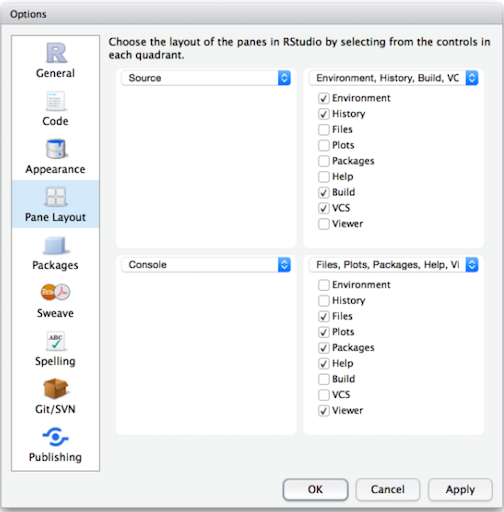
\includegraphics[width=0.6\textwidth,height=\textheight]{pane_layout.png}
\end{frame}

\begin{frame}{R Markdown}
\protect\hypertarget{r-markdown}{}
\href{https://rmarkdown.rstudio.com/}{R Markdown}

\begin{itemize}
\tightlist
\item
  R Markdown is a file format -- R Markdown files have the extension
  \textbf{.Rmd} -- that can create many kinds of static and dynamic
  documents
\item
  From \href{https://rmarkdown.rstudio.com/articles_intro.html}{RStudio}

  \begin{itemize}
  \tightlist
  \item
    ``R Markdown is a file format for making dynamic documents with R.
    An R Markdown document is written in markdown (an easy-to-write
    plain text format) and contains chunks of embedded R code''
  \end{itemize}
\item
  Examples of static documents

  \begin{itemize}
  \tightlist
  \item
    PDF documents, PDF presentations, MS word documents
  \end{itemize}
\item
  Examples of dynamic documents

  \begin{itemize}
  \tightlist
  \item
    html presentations, interactive dashboards, etc.
  \end{itemize}
\end{itemize}

How we will be using R Markdown in this class

\begin{itemize}
\tightlist
\item
  All lectures created using R Markdown
\item
  You will use R Markdown to complete homework assignments
\end{itemize}

\medskip

After this class you might:

\begin{itemize}
\tightlist
\item
  never use Microsoft Word again!
\item
  Use R Markdown to create: papers for class; presentations; journal
  manuscripts; your dissertation; etc.
\end{itemize}
\end{frame}

\begin{frame}{Why learn R? R can do a lot of stuff!}
\protect\hypertarget{why-learn-r-r-can-do-a-lot-of-stuff}{}
How we have used R+RStudio+RMarkdown in our research team

\begin{itemize}
\tightlist
\item
  Stuff traditional statistical software (e.g., SPSS, Stata) can do

  \begin{itemize}
  \tightlist
  \item
    Data manipulation, creating analysis datasets
  \item
    \href{https://ozanj.github.io/soc_of_ed_presentation/\#/slide-15}{Descriptive
    statistics and statistical models}
  \item
    Graphs
  \end{itemize}
\item
  Stuff traditional statistical software cannot do

  \begin{itemize}
  \tightlist
  \item
    \href{https://emraresearch.org/sites/default/files/2019-03/joyce_report.pdf}{Static
    policy reports}
  \item
    Static presentations

    \begin{itemize}
    \tightlist
    \item
      All lectures for this class written in RMarkdown
    \end{itemize}
  \item
    \href{https://ozanj.github.io/joyce_report/\#/title}{Interactive
    presentations}
  \item
    \href{https://ozanj.github.io/joyce_report/\#/4}{Interactive maps}
  \item
    \href{https://jkcf.shinyapps.io/dashboard/}{Interactive dashboards}
  \item
    Interactive graphs
  \end{itemize}
\end{itemize}

Some of the other stuff R can create/do:

\begin{itemize}
\tightlist
\item
  \href{https://bookdown.org/yihui/rmarkdown/websites.html}{Websites};
  \href{https://bookdown.org/yihui/rmarkdown/journals.html}{journals};
  \href{https://bookdown.org/}{books};
  \href{https://www.analyticsvidhya.com/blog/2017/03/beginners-guide-on-web-scraping-in-r-using-rvest-with-hands-on-knowledge/}{web-scraping};
  network analysis; machine learning/artificial intelligence
\end{itemize}
\end{frame}

\hypertarget{executing-r-commands}{%
\section{Executing R commands}\label{executing-r-commands}}

\begin{frame}[fragile]{R as a calculator}
\protect\hypertarget{r-as-a-calculator}{}
\begin{Shaded}
\begin{Highlighting}[]
\DecValTok{5}
\CommentTok{\#\textgreater{} [1] 5}
\DecValTok{5}\OperatorTok{+}\DecValTok{2}
\CommentTok{\#\textgreater{} [1] 7}
\DecValTok{10}\OperatorTok{*}\DecValTok{3}
\CommentTok{\#\textgreater{} [1] 30}
\end{Highlighting}
\end{Shaded}
\end{frame}

\begin{frame}[fragile]{Executing commands in R}
\protect\hypertarget{executing-commands-in-r}{}
\begin{Shaded}
\begin{Highlighting}[]
\DecValTok{5}
\CommentTok{\#\textgreater{} [1] 5}
\DecValTok{5}\OperatorTok{+}\DecValTok{2}
\CommentTok{\#\textgreater{} [1] 7}
\DecValTok{10}\OperatorTok{*}\DecValTok{3}
\CommentTok{\#\textgreater{} [1] 30}
\end{Highlighting}
\end{Shaded}

Three ways to execute commands in R

\begin{enumerate}
\tightlist
\item
  Type/copy commands directly into the ``console''
\item
  `code chunks' in RMarkdown (.Rmd files)

  \begin{itemize}
  \tightlist
  \item
    Can execute one command at a time, one chunk at a time, or ``knit''
    the entire document
  \end{itemize}
\item
  R scripts (.R files)

  \begin{itemize}
  \tightlist
  \item
    This is just a text file full of R commands
  \item
    Can execute one command at a time, several commands at a time, or
    the entire script
  \end{itemize}
\end{enumerate}
\end{frame}

\begin{frame}[fragile]{Shortcuts you should learn for executing
commands}
\protect\hypertarget{shortcuts-you-should-learn-for-executing-commands}{}
\begin{Shaded}
\begin{Highlighting}[]
\DecValTok{5}\OperatorTok{+}\DecValTok{2}
\CommentTok{\#\textgreater{} [1] 7}
\DecValTok{10}\OperatorTok{*}\DecValTok{3}
\CommentTok{\#\textgreater{} [1] 30}
\end{Highlighting}
\end{Shaded}

Three ways to execute commands in R

\begin{enumerate}
\tightlist
\item
  Type/copy commands directly into the ``console''
\item
  `code chunks' in RMarkdown (.Rmd files)

  \begin{itemize}
  \tightlist
  \item
    \textbf{Cmd/Ctrl + Enter}: execute highlighted line(s) within chunk
  \item
    \textbf{Cmd/Ctrl + Shift + k}: ``knit'' entire document
  \end{itemize}
\item
  R scripts (.R files)

  \begin{itemize}
  \tightlist
  \item
    \textbf{Cmd/Ctrl + Enter}: execute highlighted line(s)
  \item
    \textbf{Cmd/Ctrl + Shift + Enter} (without highlighting any lines):
    run entire script
  \end{itemize}
\end{enumerate}
\end{frame}

\hypertarget{r-objects-and-data-structures}{%
\section{R objects and data
structures}\label{r-objects-and-data-structures}}

\begin{frame}{Preview of lecture on objects}
\protect\hypertarget{preview-of-lecture-on-objects}{}
\begin{itemize}
\tightlist
\item
  This section of the lecture provides a conceptual and practical
  introduction to ``objects'' in R
\item
  \textbf{Important}: goal is to begin to develop familiarity with
  concepts that we will introduce in more detail in later weeks

  \begin{itemize}
  \tightlist
  \item
    I don't expect you to understand or retain all this information
    perfectly
  \item
    So just focus on understanding as much as you can and ask any
    questions that come to mind
  \end{itemize}
\end{itemize}
\end{frame}

\begin{frame}[fragile]{Assignment}
\protect\hypertarget{assignment}{}
\textbf{Assignment} refers to creating an ``object'' and assigning
values to it

\begin{itemize}
\tightlist
\item
  The object may be a variable, a dataset, a bit of text that reads ``la
  la la''
\item
  \texttt{\textless{}-} is the assignment operator

  \begin{itemize}
  \tightlist
  \item
    in other languages \texttt{=} is the assignment operator
  \end{itemize}
\item
  general syntax:

  \begin{itemize}
  \tightlist
  \item
    \texttt{object\_name\ \textless{}-\ object\_values}
  \item
    good practice to put a space before and after assignment operator
  \end{itemize}
\end{itemize}

\medskip

\begin{Shaded}
\begin{Highlighting}[]
\CommentTok{\# Create an object and assign value}
\NormalTok{a \textless{}{-}}\StringTok{ }\DecValTok{5}
\NormalTok{a}
\CommentTok{\#\textgreater{} [1] 5}

\NormalTok{b \textless{}{-}}\StringTok{ "yay!"}
\NormalTok{b}
\CommentTok{\#\textgreater{} [1] "yay!"}
\end{Highlighting}
\end{Shaded}
\end{frame}

\begin{frame}[fragile]{Objects}
\protect\hypertarget{objects}{}
R is an ``object-oriented'' programming language (like Python,
JavaScript). So, what is an ``object''?

\begin{itemize}
\tightlist
\item
  formal computer science definitions are confusing because they require
  knowledge of concepts we haven't introduced yet
\item
  More intuitively, I think objects as anything I assign values to

  \begin{itemize}
  \tightlist
  \item
    For example, below, \texttt{a} and \texttt{b} are objects I assigned
    values to
  \end{itemize}
\end{itemize}

\begin{Shaded}
\begin{Highlighting}[]
\NormalTok{a \textless{}{-}}\StringTok{ }\DecValTok{5}
\NormalTok{a}
\CommentTok{\#\textgreater{} [1] 5}
\NormalTok{b \textless{}{-}}\StringTok{ "yay!"}
\NormalTok{b}
\CommentTok{\#\textgreater{} [1] "yay!"}
\end{Highlighting}
\end{Shaded}

\begin{itemize}
\tightlist
\item
  Ben Skinner (my R maven) says ``Objects are like boxes in which we can
  put things: data, functions, and even other objects.''
\end{itemize}

Most commercial statistical software packages (e.g., SPSS, Stata)
operate on datasets, which consist of rows of observations and columns
of variables

\begin{itemize}
\tightlist
\item
  Usually, these packages can open only one dataset at a time
\item
  By contrast, in R everything is an object and there is no limit to the
  number of objects R can hold (except memory)
\end{itemize}
\end{frame}

\begin{frame}[fragile]{Vectors}
\protect\hypertarget{vectors}{}
The fundamental data structure in R is the ``vector''

\begin{itemize}
\tightlist
\item
  A vector is a collection of values
\item
  The individual values within a vector are called ``elements''
\item
  Values in a vector can be numeric, character (e.g., ``Apple''), or
  some other \emph{type}
\end{itemize}

Below we use the combine function \texttt{c()} to create a numeric
vector that contains three elements

\begin{itemize}
\tightlist
\item
  Help file says that \texttt{c()} ``combines values into a vector or
  list''
\end{itemize}

\begin{Shaded}
\begin{Highlighting}[]
\CommentTok{\#?c \# to see help file for the c() "combine" function}
\NormalTok{x \textless{}{-}}\StringTok{ }\KeywordTok{c}\NormalTok{(}\DecValTok{4}\NormalTok{, }\DecValTok{7}\NormalTok{, }\DecValTok{9}\NormalTok{) }\CommentTok{\# create object called x, which is a vector with three elements }
\CommentTok{\# (each an integer)}
\NormalTok{x }\CommentTok{\# print object x}
\CommentTok{\#\textgreater{} [1] 4 7 9}
\end{Highlighting}
\end{Shaded}

Vector where the elements are characters

\begin{Shaded}
\begin{Highlighting}[]
\NormalTok{animals \textless{}{-}}\StringTok{ }\KeywordTok{c}\NormalTok{(}\StringTok{"lions"}\NormalTok{, }\StringTok{"tigers"}\NormalTok{, }\StringTok{"bears"}\NormalTok{, }\StringTok{"oh my"}\NormalTok{) }\CommentTok{\# create object called animals}
\NormalTok{animals}
\CommentTok{\#\textgreater{} [1] "lions"  "tigers" "bears"  "oh my"}
\end{Highlighting}
\end{Shaded}
\end{frame}

\begin{frame}[fragile]{Student task}
\protect\hypertarget{student-task}{}
Either in the R console or within the R markdown file, do the following:

\begin{enumerate}
\tightlist
\item
  Create a vector called \texttt{v1} with three elements, where all the
  elements are numbers. Then print the values.
\item
  Create a vector called \texttt{v2} with four elements, where all the
  elements are characters (i.e., enclosed in single '\,' or double ""
  quotes). Then print the values.
\item
  Create a vector called \texttt{v3} with five elements, where some
  elements are numeric and some elements are characters. Then print the
  values.
\end{enumerate}
\end{frame}

\begin{frame}[fragile]{Solution to student task}
\protect\hypertarget{solution-to-student-task}{}
\begin{Shaded}
\begin{Highlighting}[]
\NormalTok{v1 \textless{}{-}}\StringTok{ }\KeywordTok{c}\NormalTok{(}\DecValTok{1}\NormalTok{, }\DecValTok{2}\NormalTok{, }\DecValTok{3}\NormalTok{) }
\CommentTok{\# create a vector called v1 with three elements}
\CommentTok{\# all the elements are numbers}
\NormalTok{v1 }\CommentTok{\# print value}
\CommentTok{\#\textgreater{} [1] 1 2 3}
\end{Highlighting}
\end{Shaded}

\begin{Shaded}
\begin{Highlighting}[]
\NormalTok{v2 \textless{}{-}}\StringTok{ }\KeywordTok{c}\NormalTok{(}\StringTok{"a"}\NormalTok{, }\StringTok{"b"}\NormalTok{, }\StringTok{"c"}\NormalTok{, }\StringTok{"d"}\NormalTok{) }
\CommentTok{\# create a vector called v2 with four elements}
\CommentTok{\# all the elements are characters}
\NormalTok{v2 }\CommentTok{\# print value}
\CommentTok{\#\textgreater{} [1] "a" "b" "c" "d"}
\end{Highlighting}
\end{Shaded}

\begin{Shaded}
\begin{Highlighting}[]
\NormalTok{v3 \textless{}{-}}\StringTok{ }\KeywordTok{c}\NormalTok{(}\DecValTok{1}\NormalTok{, }\DecValTok{2}\NormalTok{, }\DecValTok{3}\NormalTok{, }\StringTok{"a"}\NormalTok{, }\StringTok{"b"}\NormalTok{) }
\CommentTok{\# create a vector called v3 with five element}
\CommentTok{\# some elements are numeric and some elements are characters}
\NormalTok{v3 }\CommentTok{\# print value}
\CommentTok{\#\textgreater{} [1] "1" "2" "3" "a" "b"}
\end{Highlighting}
\end{Shaded}
\end{frame}

\begin{frame}{Formal classification of vectors in R}
\protect\hypertarget{formal-classification-of-vectors-in-r}{}
Here, I introduce the classification of vectors by Grolemund and Wickham

There are two broad types of vectors

\begin{enumerate}
\tightlist
\item
  \textbf{Atomic vectors}. An object that contains elements. Six
  ``types'' of atomic vectors:

  \begin{itemize}
  \tightlist
  \item
    \textbf{logical}, \textbf{integer}, \textbf{double},
    \textbf{character}, \textbf{complex}, and \textbf{raw}.

    \begin{itemize}
    \tightlist
    \item
      \textbf{Integer} and \textbf{double} vectors are collectively
      known as \textbf{numeric} vectors.
    \end{itemize}
  \end{itemize}
\item
  \textbf{Lists}. Like atomic vectors, lists are objects that contain
  elements

  \begin{itemize}
  \tightlist
  \item
    elements within a list may be atomic vectors
  \item
    elements within a list may also be other lists; that is lists can
    contain other lists
  \end{itemize}
\end{enumerate}

One difference between atomic vectors and lists: \textbf{homogeneous}
vs.~\textbf{heterogeneous} elements

\begin{itemize}
\tightlist
\item
  atomic vectors are \textbf{homogeneous}: all elements within atomic
  vector must be of the same type
\item
  lists can be \textbf{heterogeneous}: e.g., one element can be an
  integer and another element can be character
\end{itemize}
\end{frame}

\begin{frame}{Formal classification of vectors in R}
\protect\hypertarget{formal-classification-of-vectors-in-r-1}{}
Visual representation of the Grolemund and Wickham classification

\begin{figure}
\centering
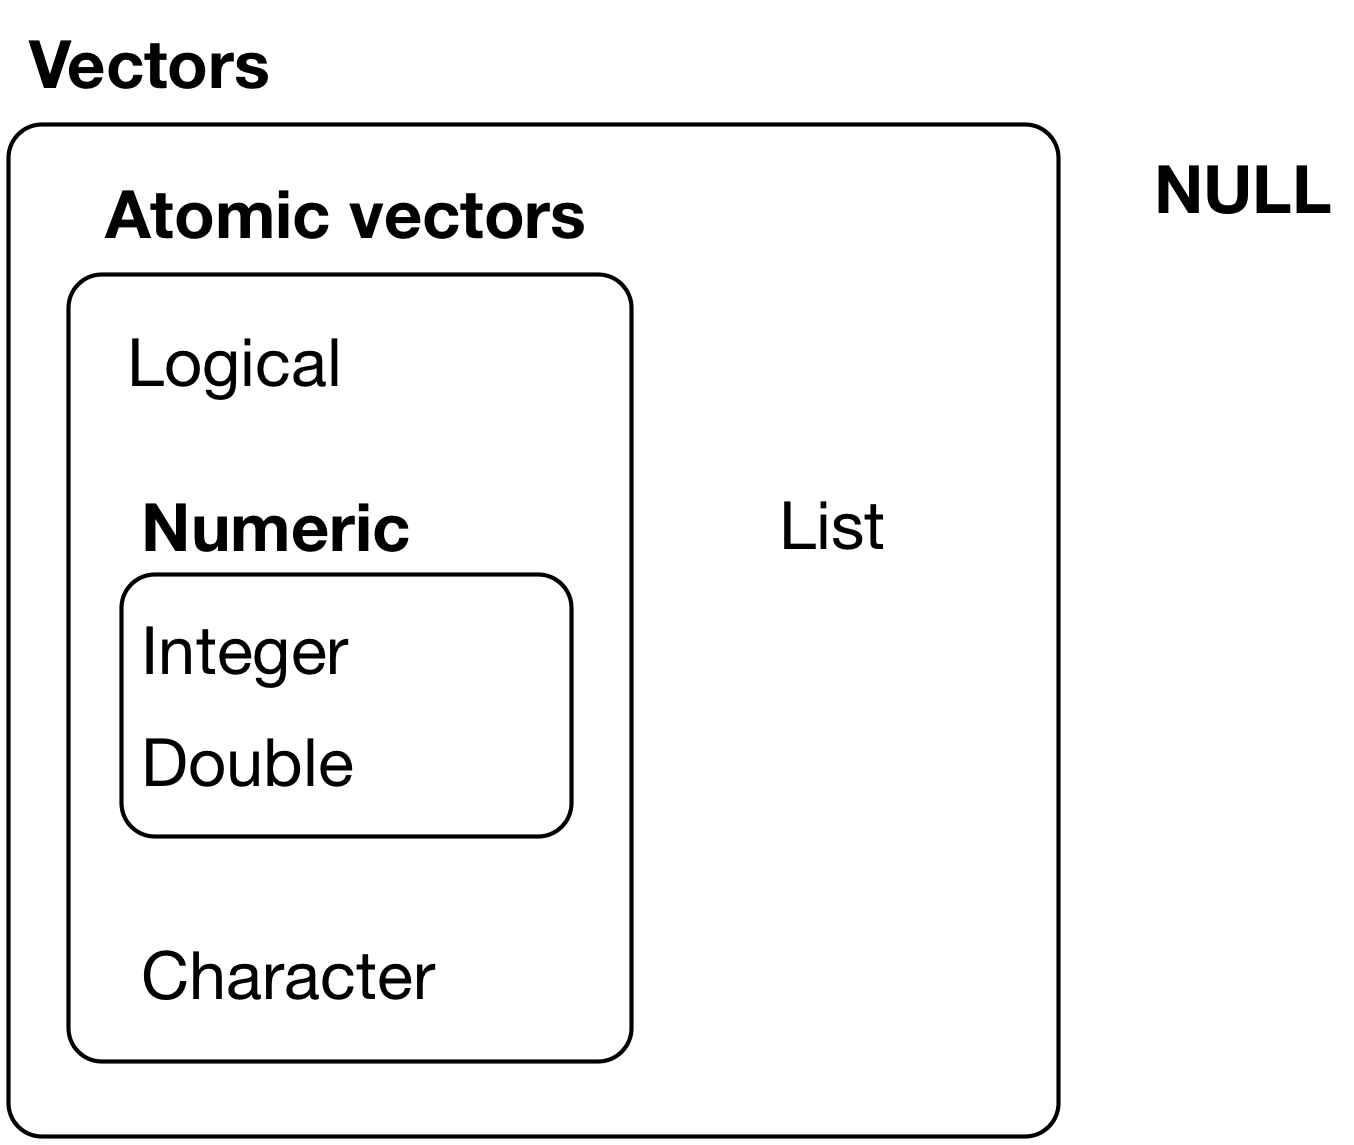
\includegraphics[width=0.6\textwidth,height=\textheight]{data-structures-overview.png}
\caption{Overview of data structures (Grolemund and Wickham, 2018,
chapter 20)}
\end{figure}
\end{frame}

\begin{frame}{Developing an intuitive understanding of vector types}
\protect\hypertarget{developing-an-intuitive-understanding-of-vector-types}{}
\textbf{Grolemund and Wickham classification}:

\begin{enumerate}
\tightlist
\item
  \textbf{Atomic vectors}. six ``types'': logical, integer, double,
  character, complex, raw.
\item
  \textbf{Lists}
\end{enumerate}

Problem with this classification:

\begin{itemize}
\tightlist
\item
  Not conceptually intutive
\item
  Technically, lists are a type of vector, but people often think of
  atomic vectors and lists as fundamentally different things
\end{itemize}

\textbf{Classification used by my R maven Ben Skinner}:

\begin{itemize}
\tightlist
\item
  data \textbf{type}: logical, numeric (integer and double), character,
  etc.
\item
  data \textbf{structure}: vector, list, matrix, etc.
\end{itemize}

I find Skinner's classification more intuitive conceptually. However, it
isn't completely consistent with how R and R functions think about
objects
\end{frame}

\hypertarget{atomic-vectors}{%
\subsection{Atomic vectors}\label{atomic-vectors}}

\begin{frame}[fragile]{``Length'' of an atomic vector is the number of
elements}
\protect\hypertarget{length-of-an-atomic-vector-is-the-number-of-elements}{}
\medskip For remainder of lecture, I'll use the term \textbf{vector} to
refer to atomic vectors

Use \texttt{length()} function to examine vector length

\begin{Shaded}
\begin{Highlighting}[]
\NormalTok{x \textless{}{-}}\StringTok{ }\KeywordTok{c}\NormalTok{(}\DecValTok{4}\NormalTok{, }\DecValTok{7}\NormalTok{, }\DecValTok{9}\NormalTok{)}
\NormalTok{x}
\CommentTok{\#\textgreater{} [1] 4 7 9}
\KeywordTok{length}\NormalTok{(x)}
\CommentTok{\#\textgreater{} [1] 3}

\NormalTok{animals \textless{}{-}}\StringTok{ }\KeywordTok{c}\NormalTok{(}\StringTok{"lions"}\NormalTok{, }\StringTok{"tigers"}\NormalTok{, }\StringTok{"bears"}\NormalTok{, }\StringTok{"oh my"}\NormalTok{)}
\NormalTok{animals}
\CommentTok{\#\textgreater{} [1] "lions"  "tigers" "bears"  "oh my"}
\KeywordTok{length}\NormalTok{(animals)}
\CommentTok{\#\textgreater{} [1] 4}
\end{Highlighting}
\end{Shaded}

A single number (or a single string/character) is a vector with
\texttt{length==1}

\begin{Shaded}
\begin{Highlighting}[]
\NormalTok{z \textless{}{-}}\StringTok{ }\DecValTok{5}
\KeywordTok{length}\NormalTok{(z)}
\CommentTok{\#\textgreater{} [1] 1}
\KeywordTok{length}\NormalTok{(}\StringTok{"Tommy"}\NormalTok{)}
\CommentTok{\#\textgreater{} [1] 1}
\end{Highlighting}
\end{Shaded}
\end{frame}

\begin{frame}[fragile]{Data type of a vector}
\protect\hypertarget{data-type-of-a-vector}{}
\medskip The ``type'' of an atomic vector refers to the elements within
the vector.

While there are six ``types'' of atomic vectors, we'll focus on the
following types:

\begin{itemize}
\tightlist
\item
  numeric:

  \begin{itemize}
  \tightlist
  \item
    ``integer'' (e.g., 5)
  \item
    ``double'' (e.g., 5.5)
  \end{itemize}
\item
  character (e.g., ``ozan'')
\item
  logical (e.g., \texttt{TRUE}, \texttt{FALSE})
\end{itemize}

Use \texttt{typeof()} function to examine vector type

\begin{Shaded}
\begin{Highlighting}[]
\NormalTok{x}
\CommentTok{\#\textgreater{} [1] 4 7 9}
\KeywordTok{typeof}\NormalTok{(x)}
\CommentTok{\#\textgreater{} [1] "double"}

\NormalTok{p \textless{}{-}}\StringTok{ }\KeywordTok{c}\NormalTok{(}\FloatTok{1.5}\NormalTok{, }\FloatTok{1.6}\NormalTok{)}
\NormalTok{p}
\CommentTok{\#\textgreater{} [1] 1.5 1.6}
\KeywordTok{typeof}\NormalTok{(p)}
\CommentTok{\#\textgreater{} [1] "double"}

\NormalTok{animals}
\CommentTok{\#\textgreater{} [1] "lions"  "tigers" "bears"  "oh my"}
\KeywordTok{typeof}\NormalTok{(animals)}
\CommentTok{\#\textgreater{} [1] "character"}
\end{Highlighting}
\end{Shaded}
\end{frame}

\begin{frame}[fragile]{Data type of a vector, numeric}
\protect\hypertarget{data-type-of-a-vector-numeric}{}
Numeric vectors can be ``integer'' (e.g., 5) or ``double'' (e.g., 5.5)

\begin{Shaded}
\begin{Highlighting}[]
\KeywordTok{typeof}\NormalTok{(}\FloatTok{1.5}\NormalTok{)}
\CommentTok{\#\textgreater{} [1] "double"}
\end{Highlighting}
\end{Shaded}

R stores numbers as doubles by default.

\begin{Shaded}
\begin{Highlighting}[]
\NormalTok{x}
\CommentTok{\#\textgreater{} [1] 4 7 9}
\KeywordTok{typeof}\NormalTok{(x)}
\CommentTok{\#\textgreater{} [1] "double"}
\end{Highlighting}
\end{Shaded}

To make an integer, place an \texttt{L} after the number:

\begin{Shaded}
\begin{Highlighting}[]
\KeywordTok{typeof}\NormalTok{(}\DecValTok{5}\NormalTok{)}
\CommentTok{\#\textgreater{} [1] "double"}
\KeywordTok{typeof}\NormalTok{(5L)}
\CommentTok{\#\textgreater{} [1] "integer"}
\end{Highlighting}
\end{Shaded}
\end{frame}

\begin{frame}[fragile]{Data type of a vector, character}
\protect\hypertarget{data-type-of-a-vector-character}{}
In contrast to ``numeric'' data types which are used to store numbers,
the ``character'' data type is used to store \textbf{strings} of text.

\begin{itemize}
\tightlist
\item
  Strings may contain any combination of numbers, letters, symbols, etc.
\item
  Character vectors are sometimes referred to as string vectors
\end{itemize}

When creating a vector where elements have \texttt{type==character} (or
when referring to the value of a string), place single `` or double ""
quotes around text

\begin{itemize}
\tightlist
\item
  the text within quotes is the ``string''
\end{itemize}

\begin{Shaded}
\begin{Highlighting}[]
\NormalTok{c1 \textless{}{-}}\StringTok{ }\KeywordTok{c}\NormalTok{(}\StringTok{"cat"}\NormalTok{,}\StringTok{\textquotesingle{}cash\textquotesingle{}}\NormalTok{,}\StringTok{\textquotesingle{}candy cane\textquotesingle{}}\NormalTok{)}
\NormalTok{c1}
\CommentTok{\#\textgreater{} [1] "cat"        "cash"       "candy cane"}
\KeywordTok{typeof}\NormalTok{(c1)}
\CommentTok{\#\textgreater{} [1] "character"}
\KeywordTok{length}\NormalTok{(c1)}
\CommentTok{\#\textgreater{} [1] 3}
\end{Highlighting}
\end{Shaded}

Numeric values can also be stored as strings

\begin{Shaded}
\begin{Highlighting}[]
\NormalTok{c2 \textless{}{-}}\StringTok{ }\KeywordTok{c}\NormalTok{(}\StringTok{"1"}\NormalTok{,}\StringTok{"2"}\NormalTok{,}\StringTok{"3"}\NormalTok{)}
\NormalTok{c2}
\CommentTok{\#\textgreater{} [1] "1" "2" "3"}
\KeywordTok{typeof}\NormalTok{(c2)}
\CommentTok{\#\textgreater{} [1] "character"}
\end{Highlighting}
\end{Shaded}
\end{frame}

\begin{frame}[fragile]{Data type of a vector, logical}
\protect\hypertarget{data-type-of-a-vector-logical}{}
Logical vectors can take three possible values: \texttt{TRUE},
\texttt{FALSE}, \texttt{NA}

\begin{itemize}
\tightlist
\item
  \texttt{TRUE}, \texttt{FALSE}, \texttt{NA} are special keywords; they
  are different from the character strings \texttt{"TRUE"},
  \texttt{"FALSE"}, \texttt{"NA"}
\item
  Don't worry about \texttt{"NA"} for now
\end{itemize}

\begin{Shaded}
\begin{Highlighting}[]
\KeywordTok{typeof}\NormalTok{(}\OtherTok{TRUE}\NormalTok{)}
\CommentTok{\#\textgreater{} [1] "logical"}
\KeywordTok{typeof}\NormalTok{(}\StringTok{"TRUE"}\NormalTok{)}
\CommentTok{\#\textgreater{} [1] "character"}

\KeywordTok{typeof}\NormalTok{(}\KeywordTok{c}\NormalTok{(}\OtherTok{TRUE}\NormalTok{,}\OtherTok{FALSE}\NormalTok{,}\OtherTok{NA}\NormalTok{))}
\CommentTok{\#\textgreater{} [1] "logical"}
\KeywordTok{typeof}\NormalTok{(}\KeywordTok{c}\NormalTok{(}\OtherTok{TRUE}\NormalTok{,}\OtherTok{FALSE}\NormalTok{,}\OtherTok{NA}\NormalTok{,}\StringTok{"FALSE"}\NormalTok{))}
\CommentTok{\#\textgreater{} [1] "character"}

\NormalTok{log \textless{}{-}}\StringTok{ }\KeywordTok{c}\NormalTok{(}\OtherTok{TRUE}\NormalTok{,}\OtherTok{TRUE}\NormalTok{,}\OtherTok{FALSE}\NormalTok{,}\OtherTok{NA}\NormalTok{,}\OtherTok{FALSE}\NormalTok{)}
\KeywordTok{typeof}\NormalTok{(log)}
\CommentTok{\#\textgreater{} [1] "logical"}
\KeywordTok{length}\NormalTok{(log)}
\CommentTok{\#\textgreater{} [1] 5}
\end{Highlighting}
\end{Shaded}

We'll learn more about logical vectors later
\end{frame}

\begin{frame}[fragile]{All elements in (atomic) vector must have same
data type.}
\protect\hypertarget{all-elements-in-atomic-vector-must-have-same-data-type.}{}
Atomic vectors are \textbf{homogenous};

\begin{itemize}
\tightlist
\item
  An atomic vector has one data type
\item
  all elements within an atomic vector must have the same data ``type''
\end{itemize}

If a vector contains elements of different type, the vector type will be
type of the most ``complex'' element

Atomic vector types from simplest to most complex:

\begin{itemize}
\tightlist
\item
  logical \textless{} integer \textless{} double \textless{} character
\end{itemize}

\begin{Shaded}
\begin{Highlighting}[]
\KeywordTok{typeof}\NormalTok{(}\KeywordTok{c}\NormalTok{(}\OtherTok{TRUE}\NormalTok{,}\OtherTok{TRUE}\NormalTok{,}\OtherTok{NA}\NormalTok{))}
\CommentTok{\#\textgreater{} [1] "logical"}

\CommentTok{\# recall L after an integer forces type to be integer }
\CommentTok{\# rather than double}
\KeywordTok{typeof}\NormalTok{(}\KeywordTok{c}\NormalTok{(}\OtherTok{TRUE}\NormalTok{,}\OtherTok{TRUE}\NormalTok{,}\OtherTok{NA}\NormalTok{,1L)) }
\CommentTok{\#\textgreater{} [1] "integer"}
\KeywordTok{typeof}\NormalTok{(}\KeywordTok{c}\NormalTok{(}\OtherTok{TRUE}\NormalTok{,}\OtherTok{TRUE}\NormalTok{,}\OtherTok{NA}\NormalTok{,}\FloatTok{1.5}\NormalTok{))}
\CommentTok{\#\textgreater{} [1] "double"}
\KeywordTok{typeof}\NormalTok{(}\KeywordTok{c}\NormalTok{(}\OtherTok{TRUE}\NormalTok{,}\OtherTok{TRUE}\NormalTok{,}\OtherTok{NA}\NormalTok{,}\FloatTok{1.5}\NormalTok{,}\StringTok{"howdy!"}\NormalTok{))}
\CommentTok{\#\textgreater{} [1] "character"}
\end{Highlighting}
\end{Shaded}
\end{frame}

\begin{frame}[fragile]{Named vectors}
\protect\hypertarget{named-vectors}{}
All vectors can be ``named'' (i.e., name individual elements within
vector)

Example of creating an unnamed vector

\begin{itemize}
\tightlist
\item
  the \texttt{str()} function ``compactly display{[}s{]} the internal
  structure of an R object'' {[}from help file{]}; very useful for
  describing objects
\end{itemize}

\begin{Shaded}
\begin{Highlighting}[]
\CommentTok{\#?str}
\NormalTok{x \textless{}{-}}\StringTok{ }\KeywordTok{c}\NormalTok{(}\DecValTok{1}\NormalTok{,}\DecValTok{2}\NormalTok{,}\DecValTok{3}\NormalTok{,}\StringTok{"hi!"}\NormalTok{)}
\NormalTok{x}
\CommentTok{\#\textgreater{} [1] "1"   "2"   "3"   "hi!"}
\KeywordTok{str}\NormalTok{(x)}
\CommentTok{\#\textgreater{}  chr [1:4] "1" "2" "3" "hi!"}
\end{Highlighting}
\end{Shaded}

Example of creating a named vector

\begin{Shaded}
\begin{Highlighting}[]
\NormalTok{y \textless{}{-}}\StringTok{ }\KeywordTok{c}\NormalTok{(}\DataTypeTok{a=}\DecValTok{1}\NormalTok{,}\DataTypeTok{b=}\DecValTok{2}\NormalTok{,}\DecValTok{3}\NormalTok{,}\DataTypeTok{c=}\StringTok{"hi!"}\NormalTok{)}
\NormalTok{y}
\CommentTok{\#\textgreater{}     a     b           c }
\CommentTok{\#\textgreater{}   "1"   "2"   "3" "hi!"}
\KeywordTok{str}\NormalTok{(y)}
\CommentTok{\#\textgreater{}  Named chr [1:4] "1" "2" "3" "hi!"}
\CommentTok{\#\textgreater{}  {-} attr(*, "names")= chr [1:4] "a" "b" "" "c"}
\end{Highlighting}
\end{Shaded}
\end{frame}

\begin{frame}[fragile]{Sequences}
\protect\hypertarget{sequences}{}
(Loose) definition: a sequence is a set of numbers in ascending or
descending order

A vector containing a ``sequence'' of numbers (e.g., 1, 2, 3) can be
created using the colon operator \texttt{:} with the notation
\texttt{start:end}

\begin{Shaded}
\begin{Highlighting}[]
\DecValTok{{-}5}\OperatorTok{:}\DecValTok{5}
\CommentTok{\#\textgreater{}  [1] {-}5 {-}4 {-}3 {-}2 {-}1  0  1  2  3  4  5}
\DecValTok{5}\OperatorTok{:{-}}\DecValTok{5}
\CommentTok{\#\textgreater{}  [1]  5  4  3  2  1  0 {-}1 {-}2 {-}3 {-}4 {-}5}
\NormalTok{s\textless{}{-}}\StringTok{ }\DecValTok{1}\OperatorTok{:}\DecValTok{10} \CommentTok{\#same as this: s\textless{}{-} c(1:10)}
\NormalTok{s}
\CommentTok{\#\textgreater{}  [1]  1  2  3  4  5  6  7  8  9 10}
\KeywordTok{length}\NormalTok{(s)}
\CommentTok{\#\textgreater{} [1] 10}
\end{Highlighting}
\end{Shaded}

Creating sequences using \texttt{seq()} function - basic syntax {[}with
default values{]}:

\begin{Shaded}
\begin{Highlighting}[]
\KeywordTok{seq}\NormalTok{(}\DataTypeTok{from =} \DecValTok{1}\NormalTok{, }\DataTypeTok{to =} \DecValTok{1}\NormalTok{, }\DataTypeTok{by =} \DecValTok{1}\NormalTok{)}
\end{Highlighting}
\end{Shaded}

\begin{Shaded}
\begin{Highlighting}[]
\KeywordTok{seq}\NormalTok{(}\DecValTok{10}\NormalTok{,}\DecValTok{15}\NormalTok{)}
\CommentTok{\#\textgreater{} [1] 10 11 12 13 14 15}
\KeywordTok{seq}\NormalTok{(}\DataTypeTok{from=}\DecValTok{10}\NormalTok{,}\DataTypeTok{to=}\DecValTok{15}\NormalTok{,}\DataTypeTok{by=}\DecValTok{1}\NormalTok{)}
\CommentTok{\#\textgreater{} [1] 10 11 12 13 14 15}
\KeywordTok{seq}\NormalTok{(}\DataTypeTok{from=}\DecValTok{100}\NormalTok{,}\DataTypeTok{to=}\DecValTok{150}\NormalTok{,}\DataTypeTok{by=}\DecValTok{10}\NormalTok{)}
\CommentTok{\#\textgreater{} [1] 100 110 120 130 140 150}
\end{Highlighting}
\end{Shaded}
\end{frame}

\begin{frame}[fragile]{Vectorized math}
\protect\hypertarget{vectorized-math}{}
Most mathematical operations operate on each element of the vector

\begin{itemize}
\tightlist
\item
  e.g., add a single value to a vector and that value will be added to
  each element of the vector
\end{itemize}

\begin{Shaded}
\begin{Highlighting}[]
\DecValTok{1}\OperatorTok{:}\DecValTok{3}
\CommentTok{\#\textgreater{} [1] 1 2 3}
\DecValTok{1}\OperatorTok{:}\DecValTok{3}\FloatTok{+.5}
\CommentTok{\#\textgreater{} [1] 1.5 2.5 3.5}
\NormalTok{(}\DecValTok{1}\OperatorTok{:}\DecValTok{3}\NormalTok{)}\OperatorTok{*}\DecValTok{2}
\CommentTok{\#\textgreater{} [1] 2 4 6}
\end{Highlighting}
\end{Shaded}

Mathematical operations involving two vectors with the same length
behave differently

\begin{itemize}
\tightlist
\item
  e.g., for addition: add element 1 of vector 1 to element 1 of vector
  2, add element 2 of vector 1 to element 2 of vector 2, etc.
\end{itemize}

\begin{Shaded}
\begin{Highlighting}[]
\KeywordTok{c}\NormalTok{(}\DecValTok{1}\NormalTok{,}\DecValTok{1}\NormalTok{,}\DecValTok{1}\NormalTok{)}\OperatorTok{+}\KeywordTok{c}\NormalTok{(}\DecValTok{1}\NormalTok{,}\DecValTok{0}\NormalTok{,}\DecValTok{2}\NormalTok{)}
\CommentTok{\#\textgreater{} [1] 2 1 3}
\KeywordTok{c}\NormalTok{(}\DecValTok{1}\NormalTok{,}\DecValTok{1}\NormalTok{,}\DecValTok{1}\NormalTok{)}\OperatorTok{*}\KeywordTok{c}\NormalTok{(}\DecValTok{1}\NormalTok{,}\DecValTok{0}\NormalTok{,}\DecValTok{2}\NormalTok{)}
\CommentTok{\#\textgreater{} [1] 1 0 2}
\end{Highlighting}
\end{Shaded}
\end{frame}

\hypertarget{lists}{%
\subsection{Lists}\label{lists}}

\begin{frame}{Lists}
\protect\hypertarget{lists-1}{}
What is a \textbf{list}?

\begin{itemize}
\tightlist
\item
  Like (atomic) vectors, a list is an object that contains
  \textbf{elements}
\item
  Unlike vectors, data types can differ across elements within a list
\item
  An element within a list can be another list

  \begin{itemize}
  \tightlist
  \item
    this characteristic makes lists more complicated than vectors
  \item
    suitable for representing hierarchical data
  \end{itemize}
\end{itemize}

Lists are more complicated than vectors; today we'll just provide a
basic introduction
\end{frame}

\begin{frame}[fragile]{Create lists using \texttt{list()} function}
\protect\hypertarget{create-lists-using-list-function}{}
Create a vector (for comparison purposes)

\begin{Shaded}
\begin{Highlighting}[]
\NormalTok{a \textless{}{-}}\StringTok{ }\KeywordTok{c}\NormalTok{(}\DecValTok{1}\NormalTok{,}\DecValTok{2}\NormalTok{,}\DecValTok{3}\NormalTok{)}
\KeywordTok{typeof}\NormalTok{(a)}
\CommentTok{\#\textgreater{} [1] "double"}
\KeywordTok{length}\NormalTok{(a)}
\CommentTok{\#\textgreater{} [1] 3}
\end{Highlighting}
\end{Shaded}

Create a list

\begin{Shaded}
\begin{Highlighting}[]
\NormalTok{b \textless{}{-}}\StringTok{ }\KeywordTok{list}\NormalTok{(}\DecValTok{1}\NormalTok{,}\DecValTok{2}\NormalTok{,}\DecValTok{3}\NormalTok{)}
\KeywordTok{typeof}\NormalTok{(b)}
\CommentTok{\#\textgreater{} [1] "list"}
\KeywordTok{length}\NormalTok{(b)}
\CommentTok{\#\textgreater{} [1] 3}
\NormalTok{b }\CommentTok{\# print list is awkward}
\CommentTok{\#\textgreater{} [[1]]}
\CommentTok{\#\textgreater{} [1] 1}
\CommentTok{\#\textgreater{} }
\CommentTok{\#\textgreater{} [[2]]}
\CommentTok{\#\textgreater{} [1] 2}
\CommentTok{\#\textgreater{} }
\CommentTok{\#\textgreater{} [[3]]}
\CommentTok{\#\textgreater{} [1] 3}
\end{Highlighting}
\end{Shaded}
\end{frame}

\begin{frame}[fragile]{Investigate structure of lists using
\texttt{str()} function}
\protect\hypertarget{investigate-structure-of-lists-using-str-function}{}
When investigating lists, \texttt{str()} is better than printing the
list

\begin{Shaded}
\begin{Highlighting}[]
\NormalTok{b \textless{}{-}}\StringTok{ }\KeywordTok{list}\NormalTok{(}\DecValTok{1}\NormalTok{,}\DecValTok{2}\NormalTok{,}\DecValTok{3}\NormalTok{)}
\KeywordTok{typeof}\NormalTok{(b)}
\CommentTok{\#\textgreater{} [1] "list"}
\KeywordTok{length}\NormalTok{(b)}
\CommentTok{\#\textgreater{} [1] 3}
\KeywordTok{str}\NormalTok{(b) }\CommentTok{\# 3 elements, each element is a numeric vector w/ length=1}
\CommentTok{\#\textgreater{} List of 3}
\CommentTok{\#\textgreater{}  $ : num 1}
\CommentTok{\#\textgreater{}  $ : num 2}
\CommentTok{\#\textgreater{}  $ : num 3}
\end{Highlighting}
\end{Shaded}

Each element of a list can be a vector of different length (i.e.,
different number of elements)

\begin{Shaded}
\begin{Highlighting}[]
\NormalTok{c \textless{}{-}}\StringTok{ }\KeywordTok{list}\NormalTok{(}\KeywordTok{c}\NormalTok{(}\DecValTok{3}\NormalTok{,}\DecValTok{4}\NormalTok{),}\KeywordTok{c}\NormalTok{(}\OperatorTok{{-}}\DecValTok{5}\NormalTok{,}\DecValTok{1}\NormalTok{,}\DecValTok{3}\NormalTok{))}
\KeywordTok{typeof}\NormalTok{(c)}
\CommentTok{\#\textgreater{} [1] "list"}
\KeywordTok{length}\NormalTok{(c)}
\CommentTok{\#\textgreater{} [1] 2}
\KeywordTok{str}\NormalTok{(c) }\CommentTok{\# 2 elements; element 1=vector w/ length=2; element 2=vector w/length=3}
\CommentTok{\#\textgreater{} List of 2}
\CommentTok{\#\textgreater{}  $ : num [1:2] 3 4}
\CommentTok{\#\textgreater{}  $ : num [1:3] {-}5 1 3}
\end{Highlighting}
\end{Shaded}
\end{frame}

\begin{frame}[fragile]{Elements within lists can have different data
types}
\protect\hypertarget{elements-within-lists-can-have-different-data-types}{}
Lists are \textbf{heterogeneous}

\begin{itemize}
\tightlist
\item
  data types can differ across elements within a list
\end{itemize}

\begin{Shaded}
\begin{Highlighting}[]
\NormalTok{b \textless{}{-}}\StringTok{ }\KeywordTok{list}\NormalTok{(}\DecValTok{1}\NormalTok{,}\DecValTok{2}\NormalTok{,}\StringTok{"apple"}\NormalTok{)}
\KeywordTok{typeof}\NormalTok{(b)}
\CommentTok{\#\textgreater{} [1] "list"}
\KeywordTok{length}\NormalTok{(b)}
\CommentTok{\#\textgreater{} [1] 3}
\KeywordTok{str}\NormalTok{(b)}
\CommentTok{\#\textgreater{} List of 3}
\CommentTok{\#\textgreater{}  $ : num 1}
\CommentTok{\#\textgreater{}  $ : num 2}
\CommentTok{\#\textgreater{}  $ : chr "apple"}
\end{Highlighting}
\end{Shaded}

Vectors are \textbf{homogeneous}

\begin{Shaded}
\begin{Highlighting}[]
\NormalTok{a \textless{}{-}}\StringTok{ }\KeywordTok{c}\NormalTok{(}\DecValTok{1}\NormalTok{,}\DecValTok{2}\NormalTok{,}\StringTok{"apple"}\NormalTok{)}
\KeywordTok{typeof}\NormalTok{(a)}
\CommentTok{\#\textgreater{} [1] "character"}
\KeywordTok{str}\NormalTok{(a)}
\CommentTok{\#\textgreater{}  chr [1:3] "1" "2" "apple"}
\end{Highlighting}
\end{Shaded}
\end{frame}

\begin{frame}[fragile]{Lists can contain other lists}
\protect\hypertarget{lists-can-contain-other-lists}{}
\begin{Shaded}
\begin{Highlighting}[]
\NormalTok{x1 \textless{}{-}}\StringTok{ }\KeywordTok{list}\NormalTok{(}\KeywordTok{c}\NormalTok{(}\DecValTok{1}\NormalTok{,}\DecValTok{2}\NormalTok{), }\KeywordTok{list}\NormalTok{(}\StringTok{"apple"}\NormalTok{, }\StringTok{"orange"}\NormalTok{), }\KeywordTok{list}\NormalTok{(}\DecValTok{1}\NormalTok{, }\DecValTok{2}\NormalTok{, }\DecValTok{3}\NormalTok{))}
\KeywordTok{str}\NormalTok{(x1)}
\CommentTok{\#\textgreater{} List of 3}
\CommentTok{\#\textgreater{}  $ : num [1:2] 1 2}
\CommentTok{\#\textgreater{}  $ :List of 2}
\CommentTok{\#\textgreater{}   ..$ : chr "apple"}
\CommentTok{\#\textgreater{}   ..$ : chr "orange"}
\CommentTok{\#\textgreater{}  $ :List of 3}
\CommentTok{\#\textgreater{}   ..$ : num 1}
\CommentTok{\#\textgreater{}   ..$ : num 2}
\CommentTok{\#\textgreater{}   ..$ : num 3}
\end{Highlighting}
\end{Shaded}

\begin{itemize}
\tightlist
\item
  first element of list is a numeric vector with length=2
\item
  second element is a list with length=2

  \begin{itemize}
  \tightlist
  \item
    first element is character vector with length=1
  \item
    second element is character vector with length=1
  \end{itemize}
\item
  third element is a list with length=3

  \begin{itemize}
  \tightlist
  \item
    first element is numeric vector with length=1
  \item
    second element is numeric vector with length=1
  \item
    third element is numeric vector with length=1
  \end{itemize}
\end{itemize}
\end{frame}

\begin{frame}[fragile]{You can name each element in the list}
\protect\hypertarget{you-can-name-each-element-in-the-list}{}
\begin{Shaded}
\begin{Highlighting}[]
\NormalTok{x2 \textless{}{-}}\StringTok{ }\KeywordTok{list}\NormalTok{(}\DataTypeTok{a=}\KeywordTok{c}\NormalTok{(}\DecValTok{1}\NormalTok{,}\DecValTok{2}\NormalTok{), }\DataTypeTok{b=}\KeywordTok{list}\NormalTok{(}\StringTok{"apple"}\NormalTok{, }\StringTok{"orange"}\NormalTok{), }\DataTypeTok{c=}\KeywordTok{list}\NormalTok{(}\DecValTok{1}\NormalTok{, }\DecValTok{2}\NormalTok{, }\DecValTok{3}\NormalTok{))}
\KeywordTok{str}\NormalTok{(x2)}
\CommentTok{\#\textgreater{} List of 3}
\CommentTok{\#\textgreater{}  $ a: num [1:2] 1 2}
\CommentTok{\#\textgreater{}  $ b:List of 2}
\CommentTok{\#\textgreater{}   ..$ : chr "apple"}
\CommentTok{\#\textgreater{}   ..$ : chr "orange"}
\CommentTok{\#\textgreater{}  $ c:List of 3}
\CommentTok{\#\textgreater{}   ..$ : num 1}
\CommentTok{\#\textgreater{}   ..$ : num 2}
\CommentTok{\#\textgreater{}   ..$ : num 3}
\end{Highlighting}
\end{Shaded}

\texttt{names()} function shows names of elements in the list

\begin{Shaded}
\begin{Highlighting}[]
\KeywordTok{names}\NormalTok{(x2) }\CommentTok{\# has names}
\CommentTok{\#\textgreater{} [1] "a" "b" "c"}
\KeywordTok{names}\NormalTok{(x1) }\CommentTok{\# no names}
\CommentTok{\#\textgreater{} NULL}
\end{Highlighting}
\end{Shaded}
\end{frame}

\begin{frame}[fragile]{Access individual elements in a ``named'' list}
\protect\hypertarget{access-individual-elements-in-a-named-list}{}
Syntax: \texttt{list\_name\$element\_name}

\begin{Shaded}
\begin{Highlighting}[]
\NormalTok{x2 \textless{}{-}}\StringTok{ }\KeywordTok{list}\NormalTok{(}\DataTypeTok{a=}\DecValTok{1}\NormalTok{, }\DataTypeTok{b=}\KeywordTok{list}\NormalTok{(}\StringTok{"apple"}\NormalTok{, }\StringTok{"orange"}\NormalTok{), }\DataTypeTok{c=}\KeywordTok{list}\NormalTok{(}\DecValTok{1}\NormalTok{, }\DecValTok{2}\NormalTok{, }\DecValTok{3}\NormalTok{))}
\NormalTok{x2}\OperatorTok{$}\NormalTok{a}
\CommentTok{\#\textgreater{} [1] 1}
\KeywordTok{typeof}\NormalTok{(x2}\OperatorTok{$}\NormalTok{a)}
\CommentTok{\#\textgreater{} [1] "double"}
\KeywordTok{length}\NormalTok{(x2}\OperatorTok{$}\NormalTok{a)}
\CommentTok{\#\textgreater{} [1] 1}

\KeywordTok{typeof}\NormalTok{(x2}\OperatorTok{$}\NormalTok{b)}
\CommentTok{\#\textgreater{} [1] "list"}
\KeywordTok{length}\NormalTok{(x2}\OperatorTok{$}\NormalTok{b)}
\CommentTok{\#\textgreater{} [1] 2}

\KeywordTok{typeof}\NormalTok{(x2}\OperatorTok{$}\NormalTok{c)}
\CommentTok{\#\textgreater{} [1] "list"}
\KeywordTok{length}\NormalTok{(x2}\OperatorTok{$}\NormalTok{c)}
\CommentTok{\#\textgreater{} [1] 3}
\end{Highlighting}
\end{Shaded}

Note: We'll spend more time practicing ``accessing elements of a list''
in upcoming weeks
\end{frame}

\begin{frame}[fragile]{Compare structure of list to structure of element
within a list}
\protect\hypertarget{compare-structure-of-list-to-structure-of-element-within-a-list}{}
\begin{Shaded}
\begin{Highlighting}[]
\KeywordTok{str}\NormalTok{(x2)}
\CommentTok{\#\textgreater{} List of 3}
\CommentTok{\#\textgreater{}  $ a: num 1}
\CommentTok{\#\textgreater{}  $ b:List of 2}
\CommentTok{\#\textgreater{}   ..$ : chr "apple"}
\CommentTok{\#\textgreater{}   ..$ : chr "orange"}
\CommentTok{\#\textgreater{}  $ c:List of 3}
\CommentTok{\#\textgreater{}   ..$ : num 1}
\CommentTok{\#\textgreater{}   ..$ : num 2}
\CommentTok{\#\textgreater{}   ..$ : num 3}

\KeywordTok{str}\NormalTok{(x2}\OperatorTok{$}\NormalTok{c)}
\CommentTok{\#\textgreater{} List of 3}
\CommentTok{\#\textgreater{}  $ : num 1}
\CommentTok{\#\textgreater{}  $ : num 2}
\CommentTok{\#\textgreater{}  $ : num 3}
\end{Highlighting}
\end{Shaded}
\end{frame}

\begin{frame}[fragile]{A DATASET IS JUST A LIST!!!!!}
\protect\hypertarget{a-dataset-is-just-a-list}{}
\medskip A data frame is a list with the following characteristics:

\begin{itemize}
\tightlist
\item
  Data type can differ across elements (like all lists)
\item
  Each element (column) is a variable
\item
  Each element in a data frame must have the same length

  \begin{itemize}
  \tightlist
  \item
    The length of an element is the number of observations (rows)
  \item
    Thus, each variable in a data frame has same number of observations
  \end{itemize}
\item
  Each element is named

  \begin{itemize}
  \tightlist
  \item
    these element names are the variable names
  \end{itemize}
\item
  Typically, each \textbf{element}(variable) in a data frame is a
  \textbf{vector}

  \begin{itemize}
  \tightlist
  \item
    Elements can also be lists. Happens when the variable has a
    complicated data structure

    \begin{itemize}
    \tightlist
    \item
      e.g., a variable that identifies the ``@'' mentions in a tweet
    \end{itemize}
  \end{itemize}
\end{itemize}

\begin{Shaded}
\begin{Highlighting}[]
\KeywordTok{names}\NormalTok{(df)}
\CommentTok{\#\textgreater{} [1] "mpg" "cyl" "hp"}
\KeywordTok{head}\NormalTok{(df, }\DataTypeTok{n=}\DecValTok{4}\NormalTok{) }\CommentTok{\# print first few rows}
\CommentTok{\#\textgreater{} \# A tibble: 4 x 3}
\CommentTok{\#\textgreater{}     mpg   cyl    hp}
\CommentTok{\#\textgreater{}   \textless{}dbl\textgreater{} \textless{}dbl\textgreater{} \textless{}dbl\textgreater{}}
\CommentTok{\#\textgreater{} 1  21       6   110}
\CommentTok{\#\textgreater{} 2  21       6   110}
\CommentTok{\#\textgreater{} 3  22.8     4    93}
\CommentTok{\#\textgreater{} 4  21.4     6   110}
\end{Highlighting}
\end{Shaded}

Additionally, data frames have ``attributes''; we'll discuss those in
upcoming weeks
\end{frame}

\begin{frame}[fragile]{A data frame is a named list}
\protect\hypertarget{a-data-frame-is-a-named-list}{}
\begin{Shaded}
\begin{Highlighting}[]
\KeywordTok{head}\NormalTok{(df, }\DataTypeTok{n=} \DecValTok{5}\NormalTok{)}
\CommentTok{\#\textgreater{} \# A tibble: 5 x 3}
\CommentTok{\#\textgreater{}     mpg   cyl    hp}
\CommentTok{\#\textgreater{}   \textless{}dbl\textgreater{} \textless{}dbl\textgreater{} \textless{}dbl\textgreater{}}
\CommentTok{\#\textgreater{} 1  21       6   110}
\CommentTok{\#\textgreater{} 2  21       6   110}
\CommentTok{\#\textgreater{} 3  22.8     4    93}
\CommentTok{\#\textgreater{} 4  21.4     6   110}
\CommentTok{\#\textgreater{} 5  18.7     8   175}
\KeywordTok{typeof}\NormalTok{(df)}
\CommentTok{\#\textgreater{} [1] "list"}
\KeywordTok{names}\NormalTok{(df)}
\CommentTok{\#\textgreater{} [1] "mpg" "cyl" "hp"}
\KeywordTok{length}\NormalTok{(df) }\CommentTok{\# length=number of variables}
\CommentTok{\#\textgreater{} [1] 3}
\KeywordTok{str}\NormalTok{(df)}
\CommentTok{\#\textgreater{} \textquotesingle{}data.frame\textquotesingle{}:    32 obs. of  3 variables:}
\CommentTok{\#\textgreater{}  $ mpg: num  21 21 22.8 21.4 18.7 18.1 14.3 24.4 22.8 19.2 ...}
\CommentTok{\#\textgreater{}  $ cyl: num  6 6 4 6 8 6 8 4 4 6 ...}
\CommentTok{\#\textgreater{}  $ hp : num  110 110 93 110 175 105 245 62 95 123 ...}
\end{Highlighting}
\end{Shaded}

Like any named list, we can examine the elements

\begin{itemize}
\tightlist
\item
  Individual elements of a data frame are the variables
\item
  these variables are vectors with length equal to the number of
  rows/observations
\end{itemize}

\begin{Shaded}
\begin{Highlighting}[]
\KeywordTok{typeof}\NormalTok{(df}\OperatorTok{$}\NormalTok{mpg)}
\CommentTok{\#\textgreater{} [1] "double"}
\KeywordTok{length}\NormalTok{(df}\OperatorTok{$}\NormalTok{mpg) }\CommentTok{\# length=number of rows/obs}
\CommentTok{\#\textgreater{} [1] 32}
\KeywordTok{str}\NormalTok{(df}\OperatorTok{$}\NormalTok{mpg)}
\CommentTok{\#\textgreater{}  num [1:32] 21 21 22.8 21.4 18.7 18.1 14.3 24.4 22.8 19.2 ...}
\end{Highlighting}
\end{Shaded}
\end{frame}

\begin{frame}[fragile]{Main takeaways about atomic vectors and lists}
\protect\hypertarget{main-takeaways-about-atomic-vectors-and-lists}{}
Basic data stuctures

\begin{enumerate}
\tightlist
\item
  \textbf{(Atomic) vectors}: \textbf{logical}, \textbf{integer},
  \textbf{double}, \textbf{character}.

  \begin{itemize}
  \tightlist
  \item
    each element in vector must have same data type
  \end{itemize}
\item
  \textbf{Lists}:

  \begin{itemize}
  \tightlist
  \item
    Data type can differ across elements
  \end{itemize}
\end{enumerate}

Takeaways

\begin{itemize}
\tightlist
\item
  These concepts are difficult; ok to feel confused
\item
  I will reinforce these concepts throughout the course
\item
  Good practice: run simple diagnostics on any new object

  \begin{itemize}
  \tightlist
  \item
    \texttt{length()} : how many \textbf{elements} in the object
  \item
    \texttt{typeof()} : what \textbf{type} of data is the object
  \item
    \texttt{str()} : hierarchical structure of the object
  \end{itemize}
\end{itemize}
\end{frame}

\begin{frame}{Main takeaways about atomic vectors and lists}
\protect\hypertarget{main-takeaways-about-atomic-vectors-and-lists-1}{}
Basic data stuctures

\begin{enumerate}
\tightlist
\item
  \textbf{(Atomic) vectors}: \textbf{logical}, \textbf{integer},
  \textbf{double}, \textbf{character}.

  \begin{itemize}
  \tightlist
  \item
    each element in vector must have same data type
  \end{itemize}
\item
  \textbf{Lists}:

  \begin{itemize}
  \tightlist
  \item
    Data type can differ across elements
  \end{itemize}
\end{enumerate}

Takeaways, continued

\begin{itemize}
\tightlist
\item
  These data structures (vectors, lists) and data types (e.g.,
  character, numeric, logical) are the basic building blocks of all
  object oriented programming languages
\item
  Application to statistical analysis

  \begin{itemize}
  \tightlist
  \item
    Datasets are just lists
  \item
    The individual elements -- columns/variables -- within a dataset are
    just vectors
  \end{itemize}
\item
  These structures and data types are foundational for all ``data
  science'' applications

  \begin{itemize}
  \tightlist
  \item
    e.g., mapping, webscraping, network analysis, etc.
  \end{itemize}
\end{itemize}
\end{frame}

\hypertarget{matrices}{%
\subsection{Matrices}\label{matrices}}

\begin{frame}[fragile]{Matrices}
\protect\hypertarget{matrices-1}{}
A \textbf{matrix} is a collection of elements arranged in a
two-dimensional rectangular layout

\begin{itemize}
\tightlist
\item
  A matrix is another ``data structure,'' in addition to vectors and
  lists
\item
  Create a matrix named \texttt{m} with 2 rows and 3 columns
\end{itemize}

\begin{Shaded}
\begin{Highlighting}[]
\NormalTok{m \textless{}{-}}\StringTok{ }\KeywordTok{matrix}\NormalTok{( }
  \KeywordTok{c}\NormalTok{(}\DecValTok{2}\NormalTok{, }\DecValTok{4}\NormalTok{, }\DecValTok{3}\NormalTok{, }\DecValTok{1}\NormalTok{, }\DecValTok{5}\NormalTok{, }\DecValTok{7}\NormalTok{), }\CommentTok{\# the data elements }
  \DataTypeTok{nrow=}\DecValTok{2}\NormalTok{,              }\CommentTok{\# number of rows }
  \DataTypeTok{ncol=}\DecValTok{3}\NormalTok{,              }\CommentTok{\# number of columns }
  \DataTypeTok{byrow =} \OtherTok{TRUE}         \CommentTok{\# fill matrix by rows }
\NormalTok{)}

\NormalTok{m }\CommentTok{\# print matrix m}
\CommentTok{\#\textgreater{}      [,1] [,2] [,3]}
\CommentTok{\#\textgreater{} [1,]    2    4    3}
\CommentTok{\#\textgreater{} [2,]    1    5    7}
\end{Highlighting}
\end{Shaded}

Investigate matrix \texttt{m}

\begin{Shaded}
\begin{Highlighting}[]
\KeywordTok{typeof}\NormalTok{(m) }\CommentTok{\# type = "double"}
\CommentTok{\#\textgreater{} [1] "double"}
\KeywordTok{str}\NormalTok{(m) }\CommentTok{\# type = numeric; has two rows and three columns}
\CommentTok{\#\textgreater{}  num [1:2, 1:3] 2 1 4 5 3 7}
\KeywordTok{class}\NormalTok{(m) }\CommentTok{\# class = matrix; more on class later}
\CommentTok{\#\textgreater{} [1] "matrix" "array"}
\end{Highlighting}
\end{Shaded}
\end{frame}

\begin{frame}[fragile]{Matrices}
\protect\hypertarget{matrices-2}{}
Like atomic vectors, matrices are homogenous data structures

\begin{Shaded}
\begin{Highlighting}[]
\NormalTok{m2 \textless{}{-}}\StringTok{ }\KeywordTok{matrix}\NormalTok{( }
  \KeywordTok{c}\NormalTok{(}\DecValTok{2}\NormalTok{, }\DecValTok{4}\NormalTok{, }\DecValTok{3}\NormalTok{, }\StringTok{"a"}\NormalTok{, }\StringTok{"b"}\NormalTok{, }\StringTok{"c"}\NormalTok{), }\CommentTok{\# the data elements }
  \DataTypeTok{nrow=}\DecValTok{2}\NormalTok{,              }\CommentTok{\# number of rows }
  \DataTypeTok{ncol=}\DecValTok{3}\NormalTok{,              }\CommentTok{\# number of columns }
  \DataTypeTok{byrow =} \OtherTok{TRUE}         \CommentTok{\# fill matrix by rows }
\NormalTok{)}

\NormalTok{m2}
\CommentTok{\#\textgreater{}      [,1] [,2] [,3]}
\CommentTok{\#\textgreater{} [1,] "2"  "4"  "3" }
\CommentTok{\#\textgreater{} [2,] "a"  "b"  "c"}
\end{Highlighting}
\end{Shaded}

Investigate matrix \texttt{m}

\begin{Shaded}
\begin{Highlighting}[]
\KeywordTok{typeof}\NormalTok{(m2) }\CommentTok{\# type = "character"}
\CommentTok{\#\textgreater{} [1] "character"}
\KeywordTok{str}\NormalTok{(m2) }\CommentTok{\# type = character; has two rows and three columns}
\CommentTok{\#\textgreater{}  chr [1:2, 1:3] "2" "a" "4" "b" "3" "c"}
\end{Highlighting}
\end{Shaded}

Why are data frames based on lists rather than matrices?

\begin{itemize}
\tightlist
\item
  a matrix is a homogenous data structure, so you couldn't have both a
  numeric variable and a character variable
\item
  a list is a heterogeneous data structure, allowing for variables of
  different underlying data types
\end{itemize}
\end{frame}

\begin{frame}{Matrices}
\protect\hypertarget{matrices-3}{}
How are matrices used in R

\begin{itemize}
\tightlist
\item
  the underlying code for statistical models uses matrices (e.g.,
  covariance matrix, matrix of regression coefficients)
\item
  For most data manipulation tasks, matrices used much less frequently
  than vectors and lists

  \begin{itemize}
  \tightlist
  \item
    In this course, we won't use matrices much at all
  \end{itemize}
\item
  Particular applications (e.g., social network analysis) make frequent
  use of matrices
\end{itemize}
\end{frame}

\begin{frame}[fragile]{Matrices}
\protect\hypertarget{matrices-4}{}
How are matrices used in R

\begin{itemize}
\tightlist
\item
  Create an ``adjacency matrix,'' which defines whether actors are
  connected to one another in a social network
\end{itemize}

\begin{Shaded}
\begin{Highlighting}[]
\NormalTok{a \textless{}{-}}\StringTok{ }\KeywordTok{matrix}\NormalTok{( }
  \KeywordTok{c}\NormalTok{(}\OtherTok{NA}\NormalTok{,}\OtherTok{NA}\NormalTok{,}\OtherTok{NA}\NormalTok{,}\OtherTok{NA}\NormalTok{,}
    \DecValTok{1}\NormalTok{,}\OtherTok{NA}\NormalTok{,}\OtherTok{NA}\NormalTok{,}\OtherTok{NA}\NormalTok{,}
    \DecValTok{1}\NormalTok{,}\DecValTok{0}\NormalTok{,}\OtherTok{NA}\NormalTok{,}\OtherTok{NA}\NormalTok{,}
    \DecValTok{0}\NormalTok{,}\DecValTok{1}\NormalTok{,}\DecValTok{0}\NormalTok{,}\OtherTok{NA}\NormalTok{), }\CommentTok{\# the data elements }
  \DataTypeTok{nrow=}\DecValTok{4}\NormalTok{,              }\CommentTok{\# number of rows }
  \DataTypeTok{ncol=}\DecValTok{4}\NormalTok{,              }\CommentTok{\# number of columns }
  \DataTypeTok{byrow =} \OtherTok{TRUE}         \CommentTok{\# fill matrix by rows }
\NormalTok{)}
\NormalTok{a\_names \textless{}{-}}\StringTok{ }\KeywordTok{c}\NormalTok{(}\StringTok{"a"}\NormalTok{,}\StringTok{"b"}\NormalTok{,}\StringTok{"c"}\NormalTok{,}\StringTok{"d"}\NormalTok{) }\CommentTok{\# create vector of actor names}
\KeywordTok{rownames}\NormalTok{(a) \textless{}{-}}\StringTok{ }\NormalTok{a\_names }\CommentTok{\# assign names to rows}
\KeywordTok{colnames}\NormalTok{(a) \textless{}{-}}\StringTok{ }\NormalTok{a\_names }\CommentTok{\# assign names to columns}
\NormalTok{a}
\CommentTok{\#\textgreater{}    a  b  c  d}
\CommentTok{\#\textgreater{} a NA NA NA NA}
\CommentTok{\#\textgreater{} b  1 NA NA NA}
\CommentTok{\#\textgreater{} c  1  0 NA NA}
\CommentTok{\#\textgreater{} d  0  1  0 NA}
\end{Highlighting}
\end{Shaded}
\end{frame}

\hypertarget{practical-example}{%
\subsection{Practical example}\label{practical-example}}

\begin{frame}[fragile]{Network data of recruiting visits from colleges
to high schools}
\protect\hypertarget{network-data-of-recruiting-visits-from-colleges-to-high-schools}{}
For this example, don't worry about understanding the code

\begin{itemize}
\tightlist
\item
  We will explain this code over coming weeks
\end{itemize}

Object \texttt{g\_2mode\_privu} contains:

\begin{itemize}
\tightlist
\item
  off-campus recruiting visits from private colleges/universities to
  private high schools
\item
  load \texttt{g\_2mode\_privu}
\end{itemize}

\begin{Shaded}
\begin{Highlighting}[]
\CommentTok{\# load igraph object of visits by private colleges/universities to private high schools}
\KeywordTok{load}\NormalTok{(}\KeywordTok{url}\NormalTok{(}\StringTok{"https://github.com/cyouh95/recruiting{-}chapter/raw/master/data/g\_2mode\_privu.rda"}\NormalTok{))}
\end{Highlighting}
\end{Shaded}

Investigate object \texttt{g\_2mode\_privu}

\begin{Shaded}
\begin{Highlighting}[]
\KeywordTok{typeof}\NormalTok{(g\_2mode\_privu) }\CommentTok{\# igraph package stores network data as type = list}
\CommentTok{\#\textgreater{} [1] "list"}
\KeywordTok{class}\NormalTok{(g\_2mode\_privu) }\CommentTok{\# class = igraph}
\CommentTok{\#\textgreater{} [1] "igraph"}
\end{Highlighting}
\end{Shaded}

The ``vertices'' consist of colleges and high schools

\begin{Shaded}
\begin{Highlighting}[]
\KeywordTok{vcount}\NormalTok{(g\_2mode\_privu) }\CommentTok{\# 1356 "nodes" or "vertices"}
\CommentTok{\#\textgreater{} [1] 1356}
\KeywordTok{table}\NormalTok{(}\KeywordTok{V}\NormalTok{(g\_2mode\_privu)}\OperatorTok{$}\NormalTok{type) }\CommentTok{\# 1330 private high schools; 26 private colleges/universities}
\CommentTok{\#\textgreater{} }
\CommentTok{\#\textgreater{} FALSE  TRUE }
\CommentTok{\#\textgreater{}  1330    26}
\end{Highlighting}
\end{Shaded}

An ``edge'' occurs when two vertices are connected to one another

\begin{itemize}
\tightlist
\item
  in \texttt{g\_2mode\_privu}, an edge occurs when a particular college
  visits a particular high school
\end{itemize}

\begin{Shaded}
\begin{Highlighting}[]
\KeywordTok{ecount}\NormalTok{(g\_2mode\_privu)}
\CommentTok{\#\textgreater{} [1] 7310}
\end{Highlighting}
\end{Shaded}
\end{frame}

\begin{frame}[fragile]{Network data of recruiting visits from colleges
to high schools}
\protect\hypertarget{network-data-of-recruiting-visits-from-colleges-to-high-schools-1}{}
An igraph object (type = list; class = igraph) can be decomposed into:

\begin{itemize}
\tightlist
\item
  a dataframe that contains characteristics (referred to as
  ``attributes'' in network literature) of the vertices
\item
  a matrix that identifies whether two vertices are connected by an edge
\end{itemize}

Create a data frame of vertex attributes

\begin{Shaded}
\begin{Highlighting}[]
\NormalTok{df\_attr \textless{}{-}}\StringTok{ }\KeywordTok{as\_data\_frame}\NormalTok{(}\DataTypeTok{x =}\NormalTok{ g\_2mode\_privu, }\DataTypeTok{what =} \StringTok{"vertices"}\NormalTok{)}

\KeywordTok{typeof}\NormalTok{(df\_attr) }\CommentTok{\# type = list}
\KeywordTok{length}\NormalTok{(df\_attr) }\CommentTok{\# length = number of variables}
\KeywordTok{class}\NormalTok{(df\_attr) }\CommentTok{\# data.frame}
\KeywordTok{str}\NormalTok{(df\_attr)}
\end{Highlighting}
\end{Shaded}
\end{frame}

\begin{frame}[fragile]{Network data of recruiting visits from colleges
to high schools}
\protect\hypertarget{network-data-of-recruiting-visits-from-colleges-to-high-schools-2}{}
Examine data frame of vertex attributes

\begin{Shaded}
\begin{Highlighting}[]
\CommentTok{\#df\_attr \%\textgreater{}\% glimpse()}
\CommentTok{\# vertices = universities}
\NormalTok{df\_attr }\OperatorTok{\%\textgreater{}\%}\StringTok{ }\KeywordTok{filter}\NormalTok{(type }\OperatorTok{==}\StringTok{ }\OtherTok{TRUE}\NormalTok{) }\OperatorTok{\%\textgreater{}\%}\StringTok{ }\KeywordTok{select}\NormalTok{(unitid,univ\_name\_ipeds,state\_code\_ipeds, classification\_ipeds)}

\CommentTok{\# vertices = high schools}
\NormalTok{df\_attr }\OperatorTok{\%\textgreater{}\%}\StringTok{ }\KeywordTok{filter}\NormalTok{(type }\OperatorTok{==}\StringTok{ }\OtherTok{FALSE}\NormalTok{) }\OperatorTok{\%\textgreater{}\%}\StringTok{ }\KeywordTok{select}\NormalTok{(ppin,name\_pss,city\_pss, state\_code\_pss)}
\end{Highlighting}
\end{Shaded}

Examine individual variables within data frame

\begin{itemize}
\tightlist
\item
  takeaway: invidividual variables within data frame are vectors!
\end{itemize}

\begin{Shaded}
\begin{Highlighting}[]
\KeywordTok{typeof}\NormalTok{(df\_attr}\OperatorTok{$}\NormalTok{name\_pss) }\CommentTok{\# vector of type = character}
\KeywordTok{str}\NormalTok{(df\_attr}\OperatorTok{$}\NormalTok{name\_pss) }\CommentTok{\# length of vector is number of obs}

\KeywordTok{typeof}\NormalTok{(df\_attr}\OperatorTok{$}\NormalTok{total\_enrolled\_pss) }\CommentTok{\# vector of type = integer}
\KeywordTok{str}\NormalTok{(df\_attr}\OperatorTok{$}\NormalTok{total\_enrolled\_pss)}
\end{Highlighting}
\end{Shaded}
\end{frame}

\begin{frame}[fragile]{Network data of recruiting visits from colleges
to high schools}
\protect\hypertarget{network-data-of-recruiting-visits-from-colleges-to-high-schools-3}{}
Create adjacency matrix of which colleges visited which high schools

\begin{Shaded}
\begin{Highlighting}[]
\NormalTok{adj\_mat \textless{}{-}}\StringTok{ }\KeywordTok{as\_adjacency\_matrix}\NormalTok{(}\DataTypeTok{graph =}\NormalTok{ g\_2mode\_privu, }\DataTypeTok{type =} \StringTok{"both"}\NormalTok{, }
                               \DataTypeTok{sparse =} \OtherTok{FALSE}\NormalTok{)}
\end{Highlighting}
\end{Shaded}

Investigate adjacency matrix

\begin{Shaded}
\begin{Highlighting}[]
\KeywordTok{typeof}\NormalTok{(adj\_mat) }\CommentTok{\# a numeric "double" object}
\CommentTok{\#\textgreater{} [1] "double"}
\KeywordTok{class}\NormalTok{(adj\_mat) }\CommentTok{\# matrix class}
\CommentTok{\#\textgreater{} [1] "matrix" "array"}
\CommentTok{\#str(adj\_mat) \# 1,356 rows by 1,356 columns}
\end{Highlighting}
\end{Shaded}

Print a few cells, visits by colleges (columns) to high schools (rows)

\begin{itemize}
\tightlist
\item
  colleges: ``\texttt{139658}'' = Emory University; ``\texttt{147767}''
  = Northwestern University; ``\texttt{152080}'' = University of Notre
  Dame
\end{itemize}

\begin{Shaded}
\begin{Highlighting}[]
\CommentTok{\#syntax: object\_name[\textless{}rows to print\textgreater{},\textless{}columns to print\textgreater{}]}
\NormalTok{adj\_mat[}\KeywordTok{c}\NormalTok{(}\StringTok{"00000226"}\NormalTok{,}\StringTok{"00000237"}\NormalTok{,}\StringTok{"00000714"}\NormalTok{),}\KeywordTok{c}\NormalTok{(}\StringTok{"139658"}\NormalTok{,}\StringTok{"147767"}\NormalTok{,}\StringTok{"152080"}\NormalTok{)]}
\CommentTok{\#\textgreater{}          139658 147767 152080}
\CommentTok{\#\textgreater{} 00000226      1      0      0}
\CommentTok{\#\textgreater{} 00000237      0      0      1}
\CommentTok{\#\textgreater{} 00000714      0      1      1}
\end{Highlighting}
\end{Shaded}
\end{frame}

\begin{frame}{Network data of recruiting visits from colleges to high
schools}
\protect\hypertarget{network-data-of-recruiting-visits-from-colleges-to-high-schools-4}{}
Plot the 2-mode network
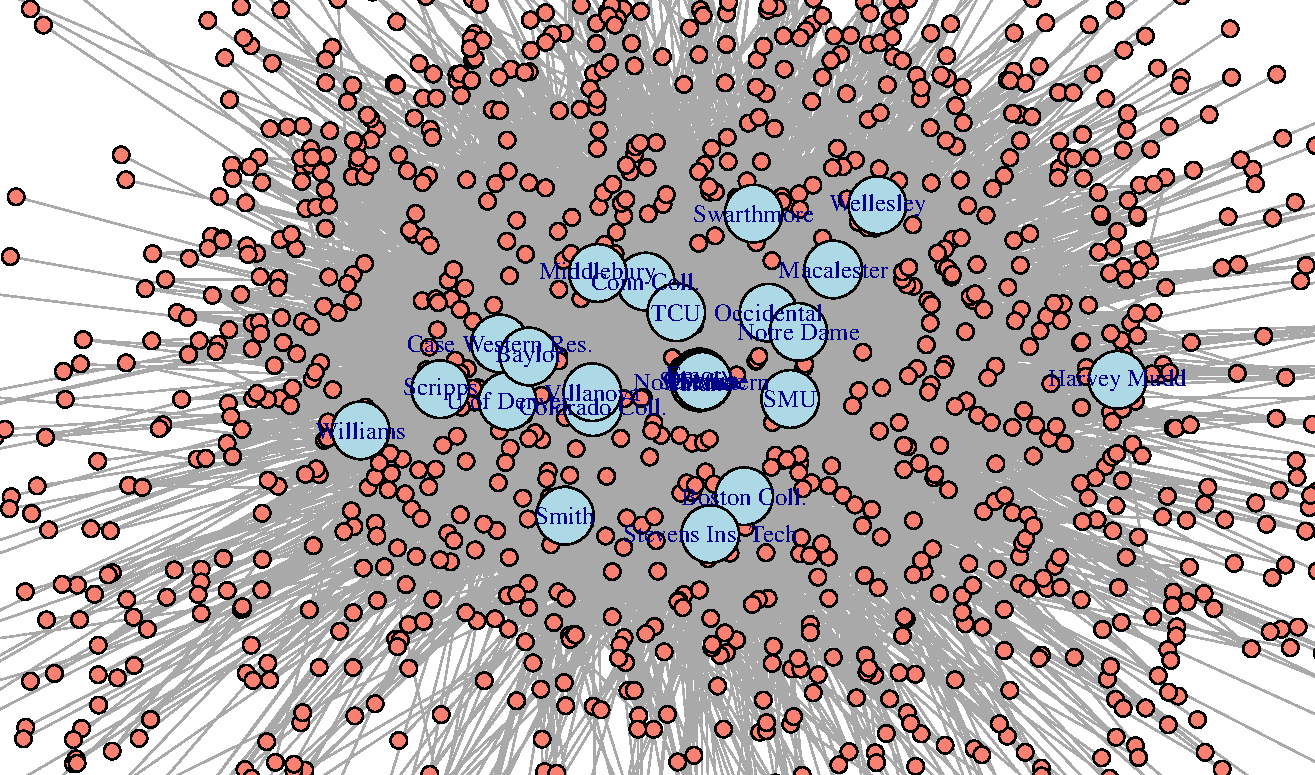
\includegraphics{intro_to_r_files/figure-beamer/unnamed-chunk-65-1.pdf}
\end{frame}

\hypertarget{using-r-functions}{%
\section{Using R functions}\label{using-r-functions}}

\begin{frame}[fragile]{What are functions}
\protect\hypertarget{what-are-functions}{}
\medskip \textbf{Functions} are pre-written bits of code that accomplish
some task.

\medskip Functions generally follow three sequential steps:

\begin{enumerate}
\tightlist
\item
  take in an \textbf{input} object(s)
\item
  \textbf{process} the input.
\item
  \textbf{return} (A) a new object or (B) a visualizatoin (e.g., plot)
\end{enumerate}

For example, \texttt{sum()} function calculates sum of elements in a
vector

\begin{enumerate}
\tightlist
\item
  \textbf{input}. takes in a vector of elements (numeric or logical)
\item
  \textbf{processing}. Calculates the sum of elements
\item
  \textbf{return}. Returns numeric vector of length=1; value is sum of
  input vector
\end{enumerate}

\begin{Shaded}
\begin{Highlighting}[]
\KeywordTok{sum}\NormalTok{(}\KeywordTok{c}\NormalTok{(}\DecValTok{1}\NormalTok{,}\DecValTok{2}\NormalTok{,}\DecValTok{3}\NormalTok{))}
\CommentTok{\#\textgreater{} [1] 6}
\KeywordTok{typeof}\NormalTok{(}\KeywordTok{sum}\NormalTok{(}\KeywordTok{c}\NormalTok{(}\DecValTok{1}\NormalTok{,}\DecValTok{2}\NormalTok{,}\DecValTok{3}\NormalTok{))) }\CommentTok{\# type of object created by sum()}
\CommentTok{\#\textgreater{} [1] "double"}
\KeywordTok{length}\NormalTok{(}\KeywordTok{sum}\NormalTok{(}\KeywordTok{c}\NormalTok{(}\DecValTok{1}\NormalTok{,}\DecValTok{2}\NormalTok{,}\DecValTok{3}\NormalTok{))) }\CommentTok{\# length of object created by sum()}
\CommentTok{\#\textgreater{} [1] 1}

\CommentTok{\#sum(c(TRUE,TRUE,FALSE))}
\CommentTok{\#typeof(sum(c(TRUE,TRUE,FALSE))); length(sum(c(TRUE,TRUE,FALSE)))}
\end{Highlighting}
\end{Shaded}
\end{frame}

\begin{frame}[fragile]{Function syntax}
\protect\hypertarget{function-syntax}{}
Components of a function

\begin{itemize}
\tightlist
\item
  function name (e.g., \texttt{sum()}, \texttt{length()},
  \texttt{seq()})
\item
  function arguments

  \begin{itemize}
  \tightlist
  \item
    Inputs that the function takes, which determine what function does

    \begin{itemize}
    \tightlist
    \item
      can be vectors, data frames, logical statements, etc.
    \end{itemize}
  \item
    In ``function call'' you specify values to assign to these function
    arguments

    \begin{itemize}
    \tightlist
    \item
      e.g., \texttt{sum(c(1,2,3))}
    \end{itemize}
  \item
    Separate arguments with a comma \texttt{,}

    \begin{itemize}
    \tightlist
    \item
      e.g., \texttt{seq(10,15)} Example: the sequence function,
      \texttt{seq()}
    \end{itemize}
  \end{itemize}
\end{itemize}

\begin{Shaded}
\begin{Highlighting}[]
\KeywordTok{seq}\NormalTok{(}\DecValTok{10}\NormalTok{,}\DecValTok{15}\NormalTok{)}
\CommentTok{\#\textgreater{} [1] 10 11 12 13 14 15}
\end{Highlighting}
\end{Shaded}
\end{frame}

\begin{frame}[fragile]{Function syntax: More on function arguments}
\protect\hypertarget{function-syntax-more-on-function-arguments}{}
Usually, function arguments have names

\begin{itemize}
\tightlist
\item
  e.g., the \texttt{seq()} function includes the arguments
  \texttt{from}, \texttt{to}, \texttt{by}
\item
  when you call the function, you need to assign values to these
  arguments; but you usually don't have to specify the name of the
  argument
\end{itemize}

\begin{Shaded}
\begin{Highlighting}[]
\KeywordTok{seq}\NormalTok{(}\DataTypeTok{from=}\DecValTok{10}\NormalTok{, }\DataTypeTok{to=}\DecValTok{20}\NormalTok{, }\DataTypeTok{by=}\DecValTok{2}\NormalTok{)}
\CommentTok{\#\textgreater{} [1] 10 12 14 16 18 20}
\KeywordTok{seq}\NormalTok{(}\DecValTok{10}\NormalTok{,}\DecValTok{20}\NormalTok{,}\DecValTok{2}\NormalTok{)}
\CommentTok{\#\textgreater{} [1] 10 12 14 16 18 20}
\end{Highlighting}
\end{Shaded}

Many function arguments have ``default values'', set by whoever wrote
the function

\begin{itemize}
\tightlist
\item
  if you don't specify a value for that argument, the default value is
  inserted
\item
  e.g., partial list of default values for \texttt{seq()}:
  \texttt{seq(from=1,\ to=1,\ by=1)}
\end{itemize}

\begin{Shaded}
\begin{Highlighting}[]
\KeywordTok{seq}\NormalTok{()}
\CommentTok{\#\textgreater{} [1] 1}
\KeywordTok{seq}\NormalTok{(}\DataTypeTok{to=}\DecValTok{10}\NormalTok{)}
\CommentTok{\#\textgreater{}  [1]  1  2  3  4  5  6  7  8  9 10}
\KeywordTok{seq}\NormalTok{(}\DecValTok{10}\NormalTok{) }\CommentTok{\# R assigned value of 10 to "to" rather than "from" or "by"}
\CommentTok{\#\textgreater{}  [1]  1  2  3  4  5  6  7  8  9 10}
\end{Highlighting}
\end{Shaded}
\end{frame}

\begin{frame}[fragile]{Function arguments, the \texttt{na.rm} argument}
\protect\hypertarget{function-arguments-the-na.rm-argument}{}
When R performs a calculation and an input has value \texttt{NA}, output
value is \texttt{NA}

\begin{Shaded}
\begin{Highlighting}[]
\DecValTok{5}\OperatorTok{+}\DecValTok{4}\OperatorTok{+}\OtherTok{NA}
\CommentTok{\#\textgreater{} [1] NA}
\end{Highlighting}
\end{Shaded}

R functions that perform calculations often have argument named
\texttt{na.rm}

\begin{itemize}
\tightlist
\item
  \texttt{na.rm} argument asks whether to remove \texttt{NA} values
  prior to calculation
\item
  For most functions, default value is \texttt{na.rm\ =\ FALSE}

  \begin{itemize}
  \tightlist
  \item
    This means ``do not remove \texttt{NAs}'' prior to calculation
  \item
    e.g., default values for \texttt{sum()} function:
    \texttt{sum(...,\ na.rm\ =\ FALSE)}
  \end{itemize}
\end{itemize}

\begin{Shaded}
\begin{Highlighting}[]
\KeywordTok{sum}\NormalTok{(}\KeywordTok{c}\NormalTok{(}\DecValTok{1}\NormalTok{,}\DecValTok{2}\NormalTok{,}\DecValTok{3}\NormalTok{,}\OtherTok{NA}\NormalTok{), }\DataTypeTok{na.rm =} \OtherTok{FALSE}\NormalTok{) }\CommentTok{\# default value}
\CommentTok{\#\textgreater{} [1] NA}
\KeywordTok{sum}\NormalTok{(}\KeywordTok{c}\NormalTok{(}\DecValTok{1}\NormalTok{,}\DecValTok{2}\NormalTok{,}\DecValTok{3}\NormalTok{,}\OtherTok{NA}\NormalTok{))}
\CommentTok{\#\textgreater{} [1] NA}
\end{Highlighting}
\end{Shaded}

\begin{itemize}
\tightlist
\item
  if you specify, \texttt{na.rm\ =\ TRUE}, \texttt{NA} values removed
  prior to calculation
\end{itemize}

\begin{Shaded}
\begin{Highlighting}[]
\KeywordTok{sum}\NormalTok{(}\KeywordTok{c}\NormalTok{(}\DecValTok{1}\NormalTok{,}\DecValTok{2}\NormalTok{,}\DecValTok{3}\NormalTok{,}\OtherTok{NA}\NormalTok{), }\DataTypeTok{na.rm =} \OtherTok{TRUE}\NormalTok{)}
\CommentTok{\#\textgreater{} [1] 6}
\end{Highlighting}
\end{Shaded}
\end{frame}

\begin{frame}[fragile]{Help files for functions}
\protect\hypertarget{help-files-for-functions}{}
To see help file on a function, type \texttt{?function\_name} without
parentheses

\begin{Shaded}
\begin{Highlighting}[]
\NormalTok{?sum}
\NormalTok{?seq}
\end{Highlighting}
\end{Shaded}

\textbf{Contents of help files}

\begin{itemize}
\tightlist
\item
  \textbf{Description}. What the function does
\item
  \textbf{Usage}. Syntax, including default values for arguments
\item
  \textbf{Arguments}. Description of function arguments
\item
  \textbf{Details}. Details and idiosyncracies of about how the function
  works.
\item
  \textbf{Value}. What (object) the function ``returns''

  \begin{itemize}
  \tightlist
  \item
    e.g., \texttt{sum()} returns vector of length 1 whose value is sum
    of input vector
  \end{itemize}
\item
  \textbf{References}. Additional reading
\item
  \textbf{See Also}. Related functions
\item
  \textbf{Examples}. Examples of function in action
\item
  Bottom of help file identifies the package the function comes from
\end{itemize}

\medskip \textbf{Practice!}

\begin{itemize}
\tightlist
\item
  when you encounter a new function, spend two minutes reading the help
  file
\item
  over time, help files will feel less cryptic and will start to feel
  helpful
\end{itemize}
\end{frame}

\begin{frame}[fragile]{Function arguments, the dot-dot-dot
(\texttt{...}) argument}
\protect\hypertarget{function-arguments-the-dot-dot-dot-...-argument}{}
\medskip On help file for many functions, you will see an argument
called \texttt{...}, referred to as the ``dot-dot-dot'' argument

\begin{Shaded}
\begin{Highlighting}[]
\NormalTok{?sum}
\NormalTok{?seq}
\end{Highlighting}
\end{Shaded}

``Dot-dot-dot'' arguments have several uses. What you should know for
now:

\begin{itemize}
\tightlist
\item
  \texttt{...} refers to arguments that are ``un-named''; but user can
  specify values

  \begin{itemize}
  \tightlist
  \item
    e.g., default syntax for \texttt{sum()}:
    \texttt{sum(...,\ na.rm\ =\ FALSE)}

    \begin{itemize}
    \tightlist
    \item
      argument \texttt{na.rm} is ``named'' (name is \texttt{na.rm});
      argument \texttt{...} un-named
    \end{itemize}
  \end{itemize}
\item
  \texttt{...} used to allow a function to take an arbitrary number of
  arguments:
\end{itemize}

\begin{Shaded}
\begin{Highlighting}[]
\CommentTok{\#Here, sum function takes 1 un{-}named argument, specifically c(10,5,NA)}
\KeywordTok{sum}\NormalTok{(}\KeywordTok{c}\NormalTok{(}\DecValTok{10}\NormalTok{,}\DecValTok{5}\NormalTok{,}\OtherTok{NA}\NormalTok{),}\DataTypeTok{na.rm=}\OtherTok{TRUE}\NormalTok{)}
\CommentTok{\#\textgreater{} [1] 15}

\CommentTok{\#Here the sum function takes 3 un{-}named arguments}
\KeywordTok{sum}\NormalTok{(}\DecValTok{10}\NormalTok{,}\DecValTok{5}\NormalTok{,}\OtherTok{NA}\NormalTok{,}\DataTypeTok{na.rm=}\OtherTok{TRUE}\NormalTok{)}
\CommentTok{\#\textgreater{} [1] 15}

\CommentTok{\#Here the sum function takes 5 un{-}named arguments}
\KeywordTok{sum}\NormalTok{(}\DecValTok{10}\NormalTok{,}\DecValTok{5}\NormalTok{,}\DecValTok{10}\NormalTok{,}\DecValTok{20}\NormalTok{,}\OtherTok{NA}\NormalTok{,}\DataTypeTok{na.rm=}\OtherTok{TRUE}\NormalTok{)}
\CommentTok{\#\textgreater{} [1] 45}
\end{Highlighting}
\end{Shaded}
\end{frame}

\hypertarget{appendix}{%
\section{Appendix}\label{appendix}}

\hypertarget{directories-and-filepaths}{%
\subsection{Directories and filepaths}\label{directories-and-filepaths}}

\begin{frame}{Directories and filepaths}
\protect\hypertarget{directories-and-filepaths-1}{}
\begin{itemize}
\tightlist
\item
  Give you a very brief overview of ``directories'' (i.e., folders) and
  ``filepaths'' (tells you where folder is located) in R
\item
  Why? After this overview we will ask you to create the directory
  structure you will use for all files related to this class
\item
  Your problem set due before class next Friday will give you more
  practice with filepaths and we have created a short document that may
  be helpful in working through this problem set
  \href{https://github.com/anyone-can-cook/rclass1/blob/master/lectures/problemset_resources/problemset_resources.pdf}{LINK}
\end{itemize}
\end{frame}

\begin{frame}[fragile]{Working directory}
\protect\hypertarget{working-directory}{}
\textbf{(Current) Working directory}

\begin{itemize}
\tightlist
\item
  The folder/directory in which you are currently working
\item
  This is where R looks for files
\item
  Files located in your current working directory can be accessed
  without specifying a filepath because R automatically looks in this
  folder
\end{itemize}

Function \texttt{getwd()} shows current working directory

\begin{Shaded}
\begin{Highlighting}[]
\KeywordTok{getwd}\NormalTok{()}
\CommentTok{\#\textgreater{} [1] "/Users/patriciamartin/Desktop/GitHub/rclass1/lectures/intro\_to\_r"}
\end{Highlighting}
\end{Shaded}

Command \texttt{list.files()} lists all files located in working
directory

\begin{Shaded}
\begin{Highlighting}[]
\KeywordTok{getwd}\NormalTok{()}
\CommentTok{\#\textgreater{} [1] "/Users/patriciamartin/Desktop/GitHub/rclass1/lectures/intro\_to\_r"}
\KeywordTok{list.files}\NormalTok{()}
\CommentTok{\#\textgreater{} [1] "data{-}structures{-}overview.png" "fp1.JPG"                     }
\CommentTok{\#\textgreater{} [3] "fp2.JPG"                      "intro\_to\_r\_files"            }
\CommentTok{\#\textgreater{} [5] "intro\_to\_r.pdf"               "intro\_to\_r.Rmd"              }
\CommentTok{\#\textgreater{} [7] "intro\_to\_r.tex"               "pane\_layout.png"             }
\CommentTok{\#\textgreater{} [9] "test.txt"}
\end{Highlighting}
\end{Shaded}
\end{frame}

\begin{frame}[fragile]{Working directory, ``Code chunks''
vs.~``console'' and ``R scripts''}
\protect\hypertarget{working-directory-code-chunks-vs.-console-and-r-scripts}{}
When you run \textbf{code chunks} in RMarkdown files (.Rmd), the working
directory is set to the filepath where the .Rmd file is stored

\begin{Shaded}
\begin{Highlighting}[]
\KeywordTok{getwd}\NormalTok{()}
\CommentTok{\#\textgreater{} [1] "/Users/patriciamartin/Desktop/GitHub/rclass1/lectures/intro\_to\_r"}
\KeywordTok{list.files}\NormalTok{()}
\CommentTok{\#\textgreater{} [1] "data{-}structures{-}overview.png" "fp1.JPG"                     }
\CommentTok{\#\textgreater{} [3] "fp2.JPG"                      "intro\_to\_r\_files"            }
\CommentTok{\#\textgreater{} [5] "intro\_to\_r.pdf"               "intro\_to\_r.Rmd"              }
\CommentTok{\#\textgreater{} [7] "intro\_to\_r.tex"               "pane\_layout.png"             }
\CommentTok{\#\textgreater{} [9] "test.txt"}
\end{Highlighting}
\end{Shaded}

When you run code from the \textbf{R Console} or an \textbf{R Script},
the working directory is your R Project directory (we'll cover this in
the next section).

Command \texttt{getwd()} shows current working directory

\begin{Shaded}
\begin{Highlighting}[]
\KeywordTok{getwd}\NormalTok{()}
\CommentTok{\#\textgreater{} [1] "/Users/patriciamartin/Desktop/GitHub/rclass1/lectures/intro\_to\_r"}
\end{Highlighting}
\end{Shaded}
\end{frame}

\begin{frame}[fragile]{Absolute vs.~relative filepath}
\protect\hypertarget{absolute-vs.-relative-filepath}{}
\textbf{Absolute file path}: The absolute file path is the complete list
of directories needed to locate a file or folder.\\
\texttt{setwd("/Users/pm/Desktop/rclass1/lectures/intro\_to\_r")}

\textbf{Relative file path}: The relative file path is the path relative
to your current location/directory. Assuming your current working
directory is in the ``intro\_to\_r'' folder and you want to change your
directory to the data folder, your relative file path would look
something like this:\\
\texttt{setwd("../../data")}

\begin{verbatim}
        File path shortcuts (Mac)
\end{verbatim}

\begin{longtable}[]{@{}ll@{}}
\toprule
\textbf{Key} & \textbf{Description}\tabularnewline
\midrule
\endhead
\textasciitilde{} & tilde is a shortcut for user's home directory (mine
is my name pm)\tabularnewline
../ & moves up a level\tabularnewline
../../ & moves up two level\tabularnewline
\bottomrule
\end{longtable}
\end{frame}

\begin{frame}{Exercise}
\protect\hypertarget{exercise}{}
\begin{enumerate}
\tightlist
\item
  Let's create a folder on our desktop and name it red\\
\item
  Inside the red folder, create two subfolders named orange and yellow\\
\item
  Inside the yellow folder create another subfolder named green
\end{enumerate}

Make sure to name these folders in lowercase.

You should have 1 folder on your desktop called red. Inside the red
folder you have two folders called orange and yellow. Inside the yellow
folder you have a folder called green.

Here is a visual of how it should look\ldots{}
\end{frame}

\begin{frame}{File path visual}
\protect\hypertarget{file-path-visual}{}
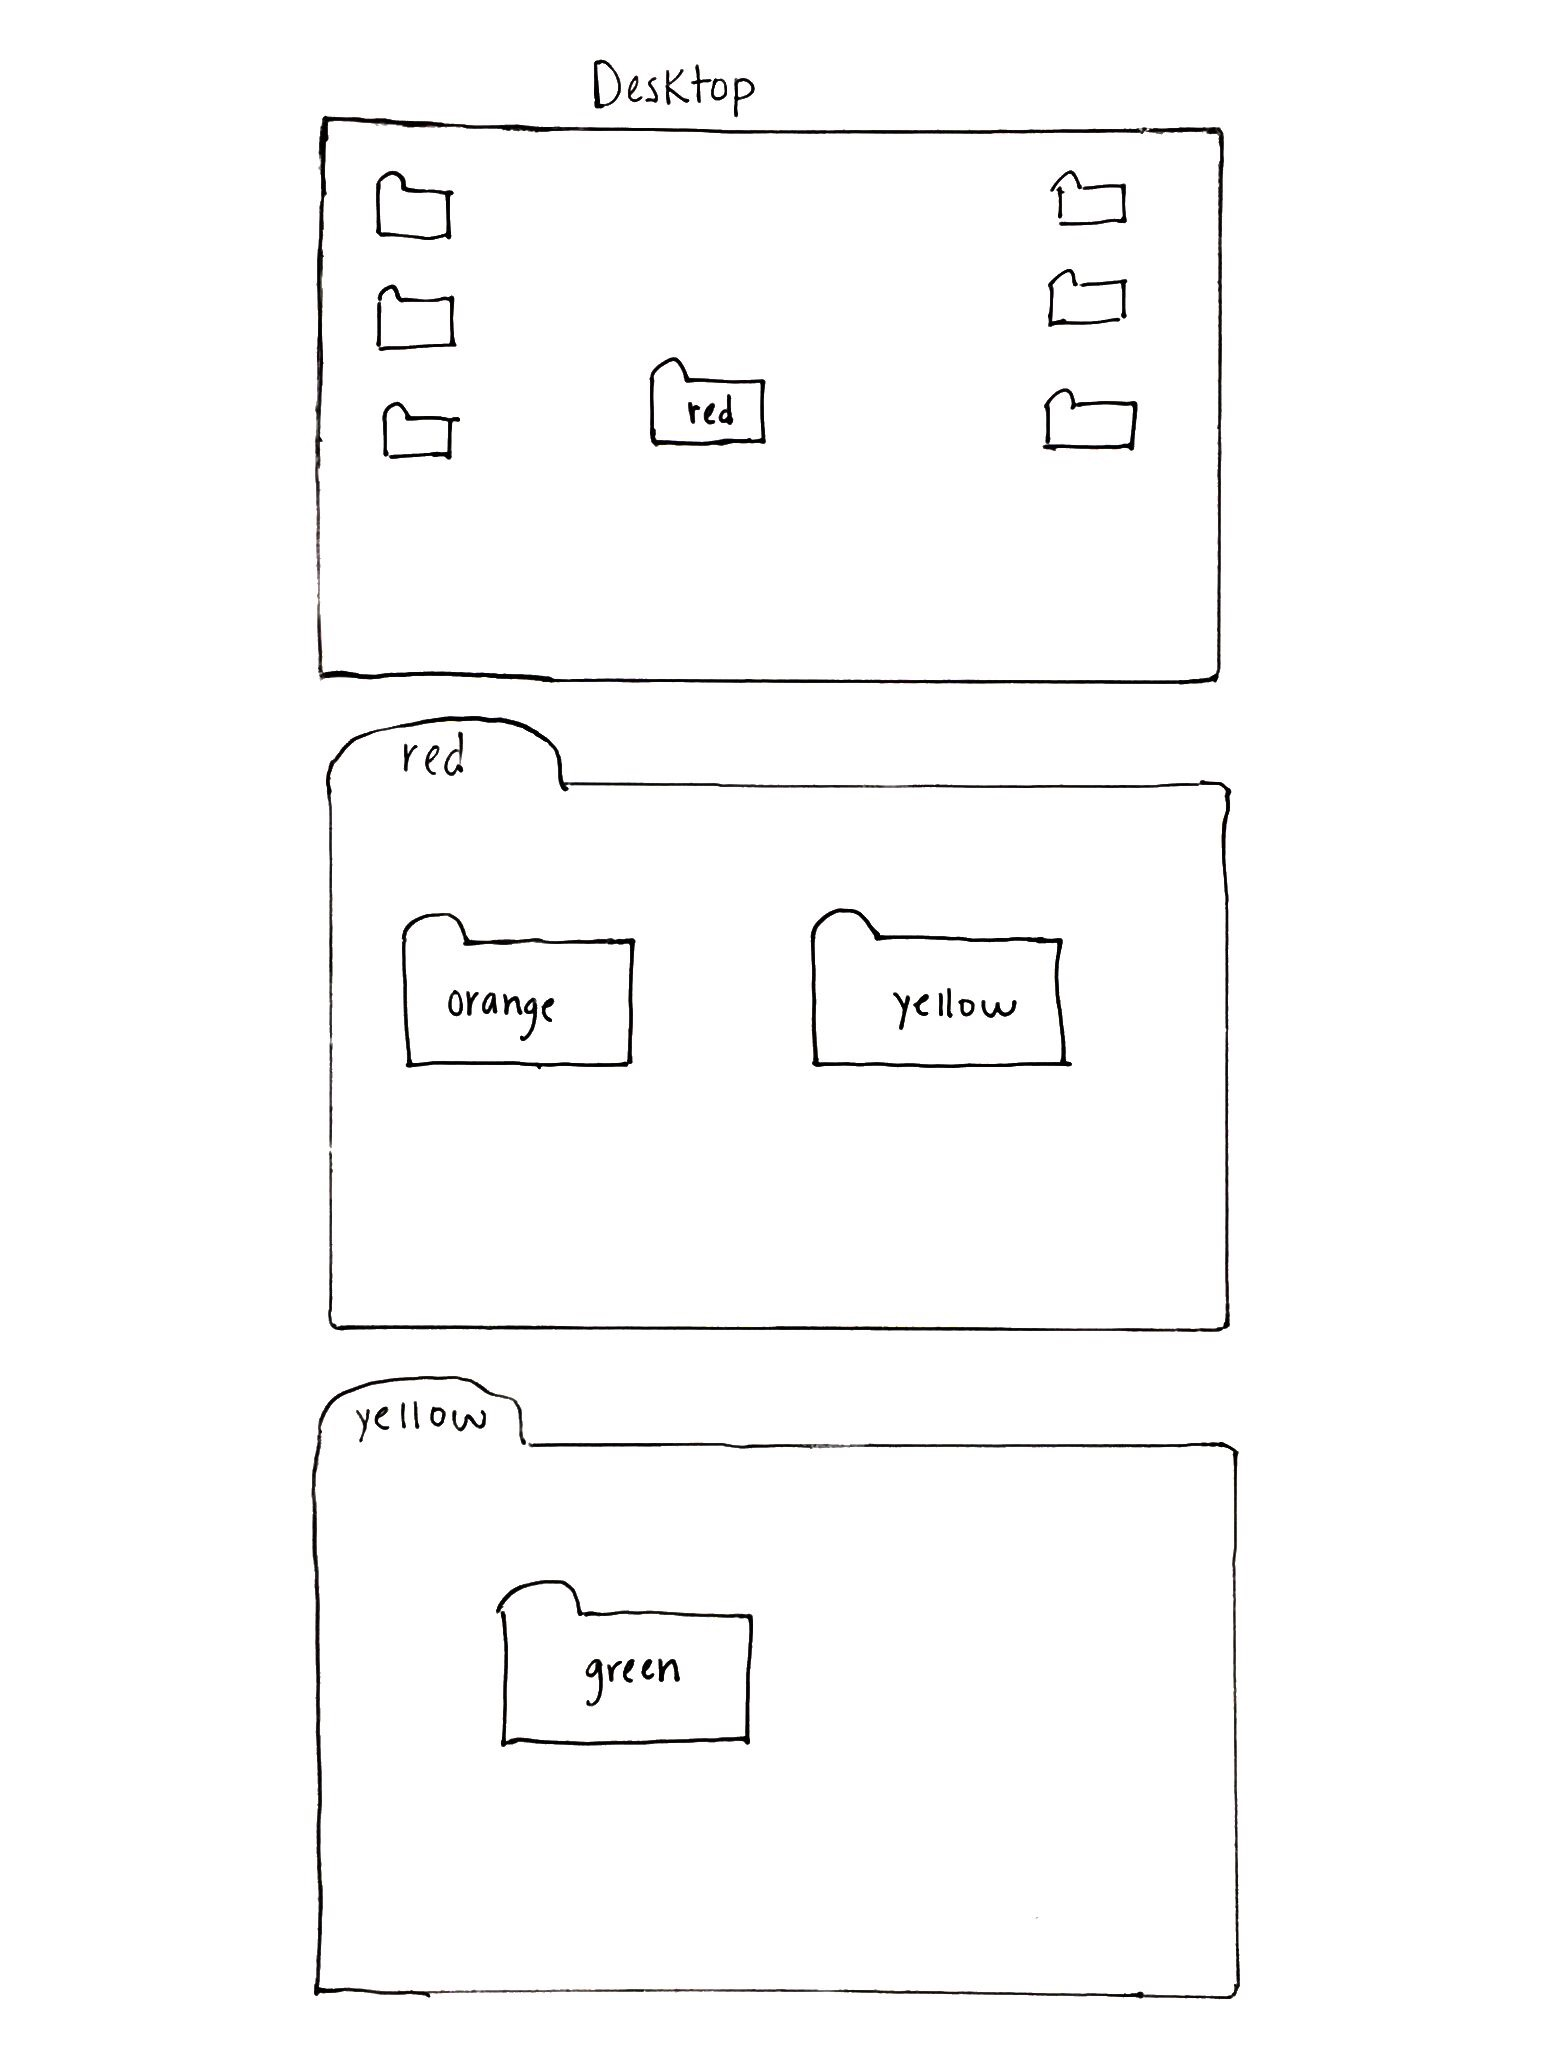
\includegraphics[width=2.08333in,height=\textheight]{fp1.JPG}
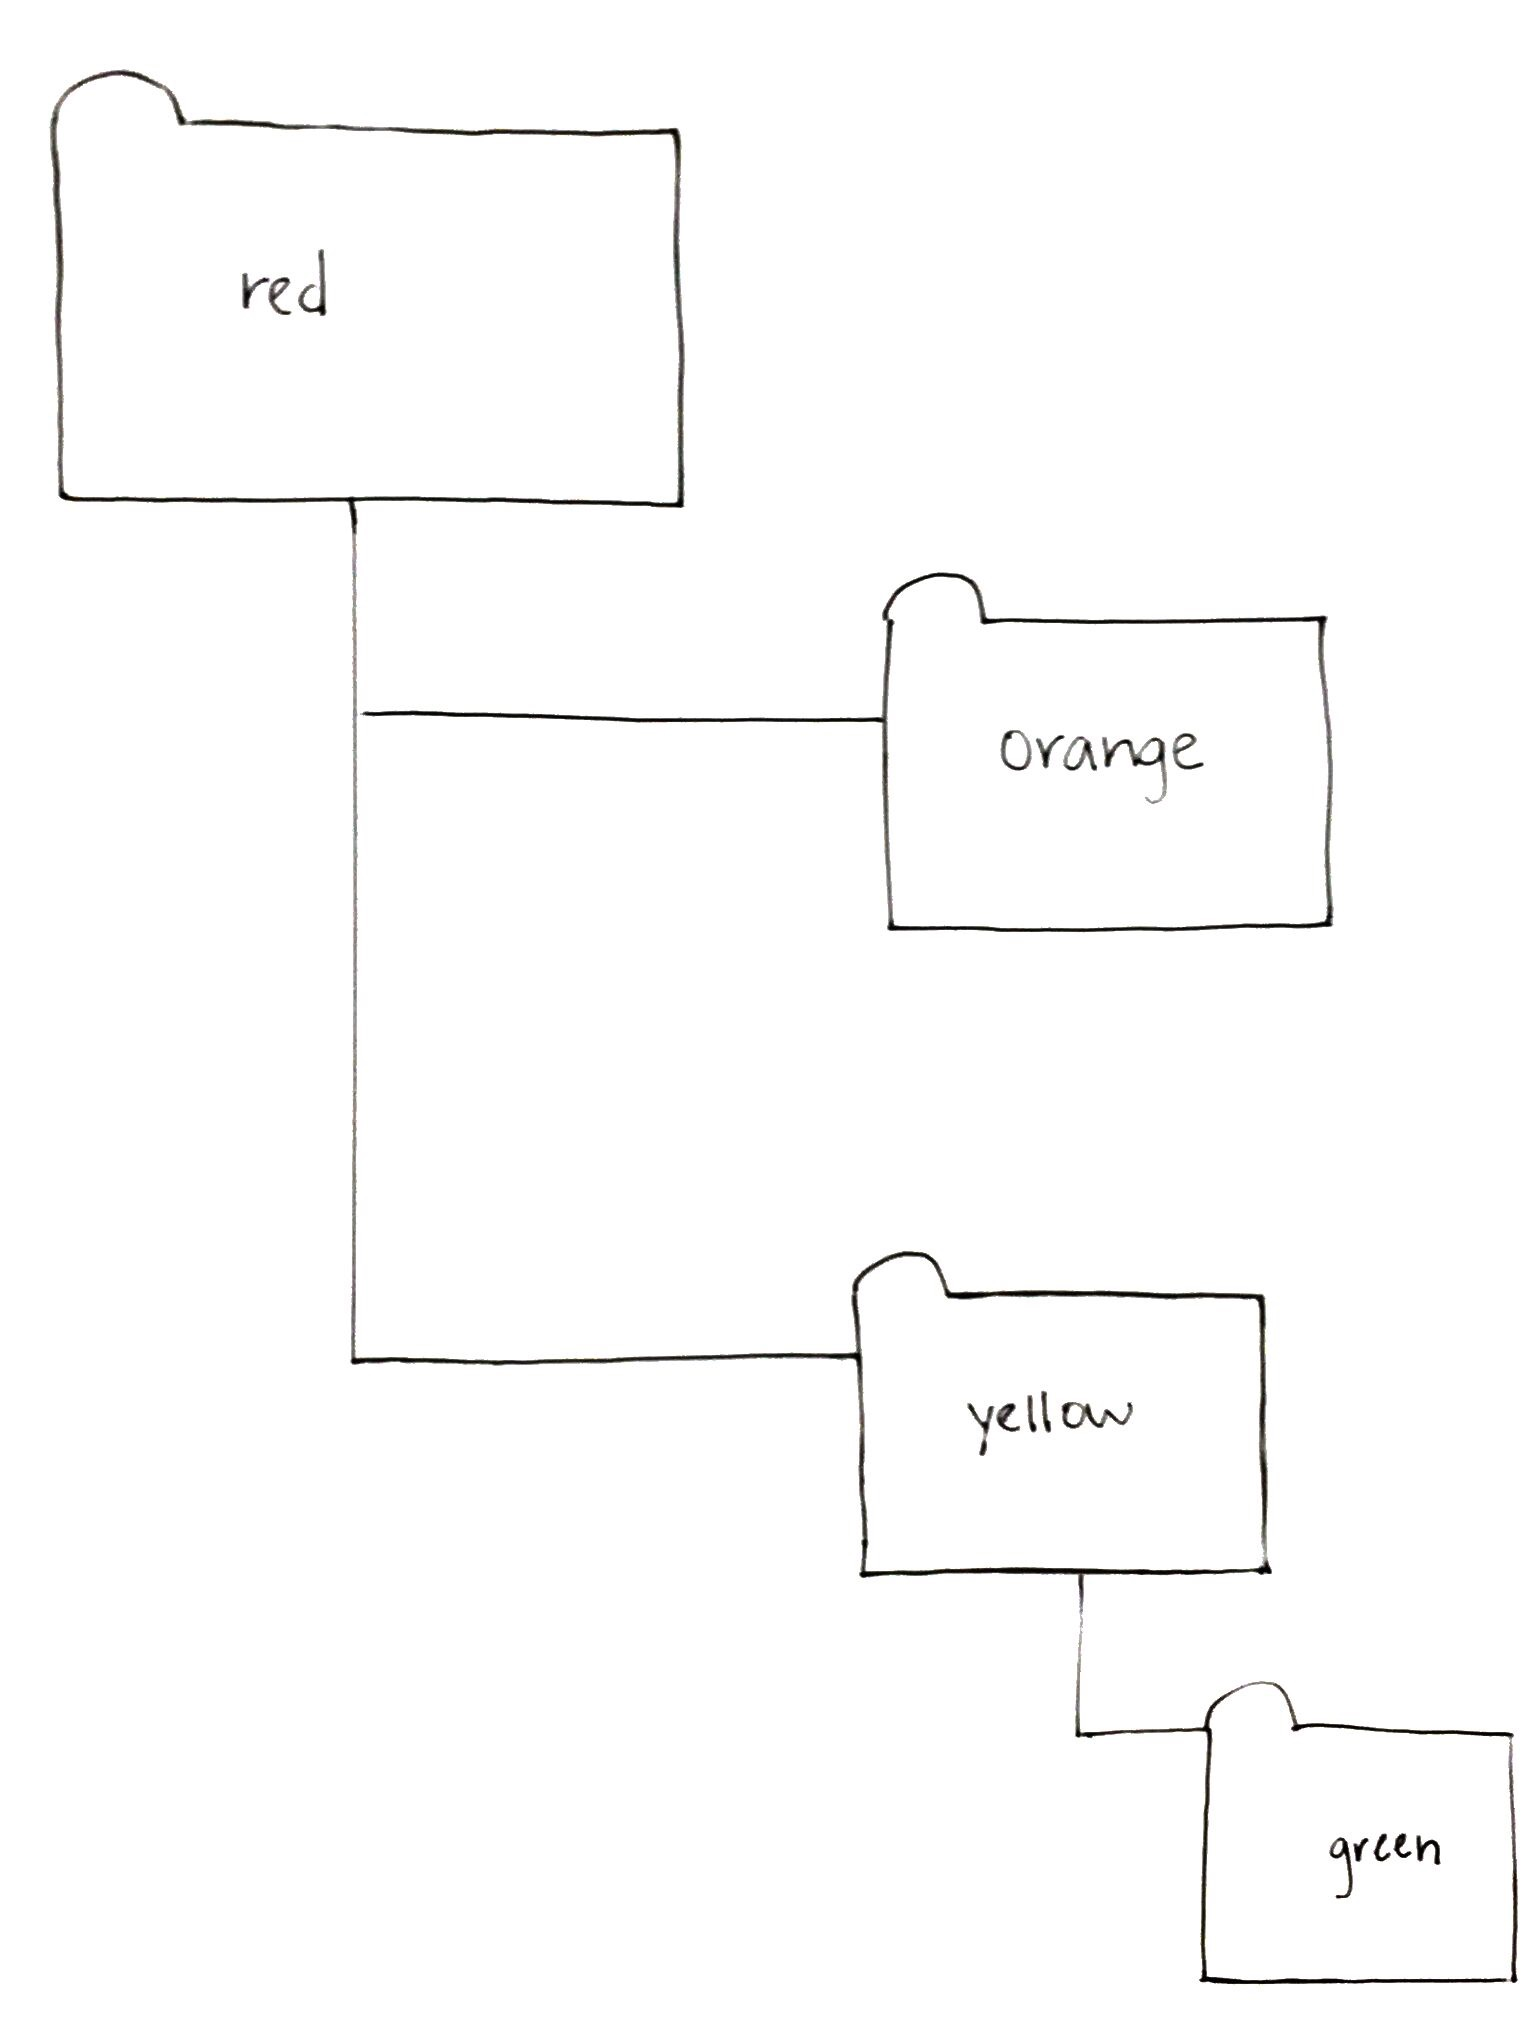
\includegraphics[width=2.08333in,height=\textheight]{fp2.JPG}
\end{frame}

\begin{frame}[fragile]{Exercise continued}
\protect\hypertarget{exercise-continued}{}
Let's say we want to get to the green folder using the absolute file
path.\\
1. View your current working directory \texttt{getwd()}\\
2. Set your working directory to the green folder using the absolute
file path\\
3. Now set your working directory to the orange folder using the
relative file path (hint: use \texttt{../})
\end{frame}

\begin{frame}[fragile]{Solution}
\protect\hypertarget{solution}{}
\begin{Shaded}
\begin{Highlighting}[]
\KeywordTok{getwd}\NormalTok{()}
\KeywordTok{setwd}\NormalTok{(}\StringTok{"\textasciitilde{}/Desktop/red/yellow/green"}\NormalTok{)}
\KeywordTok{getwd}\NormalTok{() }
\KeywordTok{setwd}\NormalTok{(}\StringTok{"../../orange"}\NormalTok{)}
\KeywordTok{getwd}\NormalTok{()}
\end{Highlighting}
\end{Shaded}
\end{frame}

\hypertarget{create-r-project-and-directory-structure}{%
\subsection{Create ``R project'' and directory
structure}\label{create-r-project-and-directory-structure}}

\begin{frame}{What is an R project? Why are you doing this?}
\protect\hypertarget{what-is-an-r-project-why-are-you-doing-this}{}
What is an ``R project''?

\begin{itemize}
\tightlist
\item
  Helps you keep all files for a project in one place
\item
  When you open an R project, the file-path of your current working
  directory is automatically set to the file-path of your R-project
\end{itemize}

Why are we asking you to create R project and download a specific
directory structure?

\begin{itemize}
\tightlist
\item
  We want you to be able to run the .Rmd files for each lecture on your
  own computer
\item
  Sometimes these .Rmd files point to certain sub-folders
\item
  If you create R project and create directory structure we recommend,
  you will be able to run .Rmd files from your own computer without
  making any changes to file-paths!
\end{itemize}
\end{frame}

\begin{frame}{Follow these steps to create ``R project'' and directory
structure}
\protect\hypertarget{follow-these-steps-to-create-r-project-and-directory-structure}{}
\begin{enumerate}
\tightlist
\item
  Download this zip folder:
  \href{https://github.com/anyone-can-cook/rclass1/blob/master/rclass1.zip}{LINK
  HERE}

  \begin{itemize}
  \tightlist
  \item
    This zip file contains the shell file directory you should use for
    this class
  \item
    Unzip the folder

    \begin{itemize}
    \tightlist
    \item
      Contains folder named ``rclass1''; this is the folder that will
      contain all materials for this course
    \item
      ``rclass1'' contains two folders: ``data'' and ``lectures''
    \end{itemize}
  \item
    Move ``rclass1'' folder to your preferred location (e.g, documents,
    desktop, dropbox, etc)
  \end{itemize}
\item
  In RStudio, click on ``File'' \textgreater\textgreater{} ``New
  Project'' \textgreater\textgreater{} ``Existing Directory''
  \textgreater\textgreater{} ``New Project''

  \begin{itemize}
  \tightlist
  \item
    ``Browse'' to find ``rclass1'' folder you just saved
  \item
    Then click on Create Project
  \end{itemize}
\item
  Save the following files in ``rclass1/lectures/intro\_to\_r''

  \begin{itemize}
  \tightlist
  \item
    intro\_to\_r.Rmd
  \item
    intro\_to\_r.pdf
  \end{itemize}
\end{enumerate}
\end{frame}

\begin{frame}{Next, you follow these steps}
\protect\hypertarget{next-you-follow-these-steps}{}
\begin{itemize}
\tightlist
\item
  You can add any additional sub-folders you want to the ``rclass1''
  folder

  \begin{itemize}
  \tightlist
  \item
    e.g., ``syllabus'', ``resources''
  \end{itemize}
\item
  You can add any additional files you want to the sub-directory folders
  you unzipped

  \begin{itemize}
  \tightlist
  \item
    e.g., in ``rclass1/lectures/intro\_to\_r'' you might add an
    additional document of notes you took
  \end{itemize}
\end{itemize}
\end{frame}

\hypertarget{r-markdown-1}{%
\subsection{R Markdown}\label{r-markdown-1}}

\begin{frame}[fragile]{What is R Markdown}
\protect\hypertarget{what-is-r-markdown}{}
\begin{itemize}
\tightlist
\item
  R Markdown documents embed R code, output associated with R code, and
  text into one document
\item
  An R Markdown document is a ``\,`Living' document that updates every
  time you compile {[}"knit"{]} it''
\item
  R Markdown documents have the extension .Rmd

  \begin{itemize}
  \tightlist
  \item
    Can think of them as text files with the extension .Rmd rather than
    .txt
  \end{itemize}
\item
  At top of .Rmd file you specify the ``output'' style, which dictates
  what kind of formatted document will be created

  \begin{itemize}
  \tightlist
  \item
    e.g., \texttt{html\_document} or \texttt{pdf\_document}
  \end{itemize}
\item
  When you compile {[}``knit''{]} a .Rmd file, the resulting formatted
  document can be an HTML document, a PDF document, an MS Word document,
  or many other types
\end{itemize}

\emph{This slide borrows from Darin Christensen}
\end{frame}

\begin{frame}[fragile]{How people use R Markdown}
\protect\hypertarget{how-people-use-r-markdown}{}
R Markdown creates many types of static and dynamic/interactive
documents

\begin{itemize}
\tightlist
\item
  Example of
  \href{https://emraresearch.org/sites/default/files/2019-03/joyce_report.pdf}{static
  policy report}
\item
  Example of
  \href{https://ozanj.github.io/joyce_report/\#/title}{dynamic/interactive
  presentation}
\end{itemize}

How I use R Markdown

\begin{itemize}
\tightlist
\item
  Journal manuscripts; reports; presentations; for taking notes when I
  am learning new methods or reading an empirical paper
\end{itemize}

How we will be using R Markdown files in this class:

\begin{itemize}
\tightlist
\item
  Homework you submit will be .Rmd files, where ``output'' style will be
  \texttt{html\_document} or \texttt{pdf\_document}
\item
  Lectures we write are .Rmd files, where the output style will be
  \texttt{beamer\_presentation} or \texttt{html\_document}

  \begin{itemize}
  \tightlist
  \item
    \texttt{beamer\_presentation} is essentially a PDF document, where
    each page is a slide
  \end{itemize}
\end{itemize}
\end{frame}

\begin{frame}{Creating R Markdown documents}
\protect\hypertarget{creating-r-markdown-documents}{}
\textbf{Do this with a partner}

Approach for creating a RMarkdown document.

\begin{enumerate}
\tightlist
\item
  Point-and-click from within RStudio

  \begin{itemize}
  \tightlist
  \item
    Click on \emph{File} \textgreater\textgreater{} \emph{New File}
    \textgreater\textgreater{} \emph{R Markdown}
    \textgreater\textgreater{} \emph{Document}
    \textgreater\textgreater{} choose \emph{HTML}
    \textgreater\textgreater{} click \emph{OK}

    \begin{itemize}
    \tightlist
    \item
      Optional: add title (this is not the file name, just what appears
      at the top of document)
    \item
      Optional: add author name
    \end{itemize}
  \item
    Save the .Rmd file; \emph{File} \textgreater\textgreater{}
    \emph{Save As}

    \begin{itemize}
    \tightlist
    \item
      Any file name
    \item
      Recommend you save it in same folder you saved this lecture
    \end{itemize}
  \item
    ``Knit'' the entire .Rmd file

    \begin{itemize}
    \tightlist
    \item
      Point-and-click OR shortcut: \textbf{Cmd/Ctrl + Shift + k}
    \end{itemize}
  \end{itemize}
\end{enumerate}
\end{frame}

\begin{frame}[fragile]{Components of a .Rmd file}
\protect\hypertarget{components-of-a-.rmd-file}{}
An R Markdown (.Rmd) file consists of several parts

\begin{enumerate}
\tightlist
\item
  \textbf{YAML header}

  \begin{itemize}
  \tightlist
  \item
    YAML stands for ``yet another markup language''
  \item
    Controls settings that apply to the whole document (e.g., ``output''
    should be \texttt{html\_document} or \texttt{pdf\_document}, whether
    to include table of contents, etc.)
  \item
    YAML header goes at the very top of the document
  \item
    Starts with a line of three horizontal dashes \texttt{-\/-\/-}; ends
    with a line of three horizontal dashes \texttt{-\/-\/-}
  \end{itemize}
\item
  \textbf{Text} in body of .Rmd file

  \begin{itemize}
  \tightlist
  \item
    e.g., headings; description of results, etc.
  \end{itemize}
\item
  \textbf{R code chunks} in body of .Rmd file
\end{enumerate}

\begin{Shaded}
\begin{Highlighting}[]
\NormalTok{a \textless{}{-}}\StringTok{ }\KeywordTok{c}\NormalTok{(}\DecValTok{2}\NormalTok{,}\DecValTok{4}\NormalTok{,}\DecValTok{6}\NormalTok{)}
\NormalTok{a}
\NormalTok{a}\DecValTok{{-}1}
\end{Highlighting}
\end{Shaded}

\begin{enumerate}
\setcounter{enumi}{3}
\tightlist
\item
  \textbf{R output} associated with code chunks
\end{enumerate}

\begin{verbatim}
#> [1] 2 4 6
#> [1] 1 3 5
\end{verbatim}
\end{frame}

\begin{frame}{Comment: Running R code chunks vs.~``knit'' entire .Rmd
file}
\protect\hypertarget{comment-running-r-code-chunks-vs.-knit-entire-.rmd-file}{}
Two ways to execute R commands in .Rmd file:

\begin{enumerate}
\tightlist
\item
  ``Knit'' entire .Rmd file

  \begin{itemize}
  \tightlist
  \item
    shortcut: \textbf{Cmd/Ctrl + Shift + k}
  \end{itemize}
\item
  ``Run'' code chunk or selected lines within code chunk

  \begin{itemize}
  \tightlist
  \item
    Run selected line(s): \textbf{Cmd/Ctrl + Enter}
  \item
    Run current chunk: \textbf{Cmd/Ctrl + Shift + Enter}
  \end{itemize}
\end{enumerate}

Comment on default settings for RStudio:

\begin{itemize}
\tightlist
\item
  When you knit entire .Rmd file, ``objects'' created within .Rmd file
  will not be available after file compiles
\item
  When you run code chunk (or selected lines in chunk), objects created
  by lines you run will be in your ``environment'' until you remove them
  or quit R session
\end{itemize}
\end{frame}

\begin{frame}[fragile]{Output types of .Rmd file}
\protect\hypertarget{output-types-of-.rmd-file}{}
Common/important output types:

\begin{itemize}
\tightlist
\item
  \textbf{html\_document}: R Markdown originally designed to create HTML
  documents

  \begin{itemize}
  \tightlist
  \item
    Most features/code in .Rmd files were written for html\_document
  \item
    Many of these features are available in other output types
  \item
    When learning R Markdown, best to start by learning html\_document
  \end{itemize}
\item
  \textbf{pdf\_document}: Requires installation of \texttt{tinytex} R
  package or LaTeX (MiKTeX/MacTeX)

  \begin{itemize}
  \tightlist
  \item
    How it works:

    \begin{itemize}
    \tightlist
    \item
      You write .Rmd code
    \item
      When you compile, this .Rmd code is transformed into LaTeX code
    \item
      LaTeX ``engine'' creates the formatted .pdf file
    \end{itemize}
  \item
    Can include some of the same features available for
    \emph{html\_document}
  \item
    Can insert LaTeX commands in .Rmd file with \emph{pdf\_document}
    output
  \end{itemize}
\item
  \textbf{beamer\_presentation}: Requires installation of LaTeX

  \begin{itemize}
  \tightlist
  \item
    ``beamer'' is the name for presentations written in LaTeX
  \item
    Essentially creates PDF of presentation slides
  \item
    Lectures for this class created with \emph{beamer\_presentation}
    output
  \item
    Note: YAML header includes \texttt{beamer\_header.tex} file, which
    creates some formatting rules and additional commands
  \end{itemize}
\end{itemize}
\end{frame}

\begin{frame}{Learning more about R Markdown}
\protect\hypertarget{learning-more-about-r-markdown}{}
Resources

\begin{itemize}
\tightlist
\item
  Cheat sheets and quick reference:

  \begin{itemize}
  \tightlist
  \item
    \href{https://www.rstudio.com/wp-content/uploads/2015/02/rmarkdown-cheatsheet.pdf}{Cheat
    Sheet}
  \item
    \href{https://www.rstudio.com/wp-content/uploads/2015/03/rmarkdown-reference.pdf}{Quick
    Reference} {[}I prefer the quick reference{]}
  \end{itemize}
\item
  Chapters/books

  \begin{itemize}
  \tightlist
  \item
    \href{http://r4ds.had.co.nz/r-markdown.html}{Chapter 27} of ``R for
    Data Science'' book
  \item
    \href{https://bookdown.org/yihui/rmarkdown/}{R Markdown: The
    Definative Guide} book {[}I prefer this book{]}
  \end{itemize}
\end{itemize}

How you will learn R Markdown

\begin{itemize}
\tightlist
\item
  Lectures written as .Rmd file

  \begin{itemize}
  \tightlist
  \item
    During class run ``code chunks'' and try to ``knit'' entire .Rmd
    file
  \end{itemize}
\item
  I'll assign \textbf{small} amount of reading on R Markdown

  \begin{itemize}
  \tightlist
  \item
    Prior to next week:

    \begin{itemize}
    \tightlist
    \item
      Spend 15 minutes familiarizing yourself with
      \href{https://www.rstudio.com/wp-content/uploads/2015/03/rmarkdown-reference.pdf}{Quick
      Reference}
    \item
      Read section
      \href{https://bookdown.org/yihui/rmarkdown/html-document.html}{3.1
      of R Markdown: The Definative Guide}, about creating
      html\_document
    \end{itemize}
  \end{itemize}
\item
  Homework must be written in .Rmd file

  \begin{itemize}
  \tightlist
  \item
    You will submit .Rmd file AND output of compiled file
  \item
    For next week, you will submit homework as html\_document output
  \end{itemize}
\end{itemize}
\end{frame}

\begin{frame}[fragile]{Directory structure for this class}
\protect\hypertarget{directory-structure-for-this-class}{}
In order to be able to ``knit'' entire lectures {[}rather than just run
specific code chunks{]} make sure that you have the following directory
structure:

\begin{itemize}
\tightlist
\item
  rclass1

  \begin{itemize}
  \tightlist
  \item
    lectures

    \begin{itemize}
    \tightlist
    \item
      intro\_to\_r/
    \item
      \ldots{}
    \item
      join\_data/
    \item
      beamer\_header.tex
    \end{itemize}
  \end{itemize}
\end{itemize}

What is beamer\_header.tex?

\begin{itemize}
\tightlist
\item
  A text file that contains \LaTeX code
\item
  This code creates formatting rules that are applied to all lecture
  slides
\item
  If you go YAML header you will see:
\end{itemize}

\begin{Shaded}
\begin{Highlighting}[]
\NormalTok{    includes}\OperatorTok{:}
\StringTok{      }\NormalTok{in\_header}\OperatorTok{:}\StringTok{ }\NormalTok{..}\OperatorTok{/}\NormalTok{beamer\_header.tex}
\end{Highlighting}
\end{Shaded}

\begin{itemize}
\tightlist
\item
  This runs beamer\_header.tex; assumes that beamer\_header.tex is
  located one level up from your current directory
\item
  If you don't have beamer\_header.tex saved to appropriate place, you
  can download it here
  \href{https://github.com/anyone-can-cook/rclass1/blob/master/lectures/beamer_header.tex}{LINK}
\item
  Note: we may revise beamer\_header.tex as we work out formatting bugs
\end{itemize}
\end{frame}

\end{document}
